\mychapter{MCTest versões 4, 4.G e 5}\label{ch:experimentos_QR_QT}

Neste capítulo, são apresentadas as versões adicionais do MCTest, nomeadamente o MCTest-4, MCTest-4.G e MCTest-5.

O MCTest-4 é um software desenvolvido para a \textbf{correção} de exames com QMs. Ele lê um arquivo PDF contendo os QRs dos estudantes, identifica automaticamente cada estudante utilizando código de barras e corrige exames individuais com questões e alternativas aleatórias.  O programa realiza a correção dos exames comparando as respostas marcadas com o gabarito e gera um arquivo CSV contendo a correção de cada questão, bem como o número total de questões corretas e inválidas.

O MCTest-4.G (de \textit{generate}) é um software desenvolvido para a \textbf{geração} de exames com questões. Ele lê uma estrutura de pastas e arquivos contendo dados de estudantes e matrícula, além de um banco de QMs ou QTs. O MCTest-4.G utiliza esses dados para gerar exames distintos e aleatórios para cada estudante. Nas folhas de exame, além do nome e matrícula do estudante, há um código de barras referente à sua matrícula.

Além disso, neste capítulo, são apresentados os experimentos conduzidos na versão mais recente, o MCTest-5, que agora é baseado na web e usa o banco de dados MySQL. No entanto, a integração com as atividades VPL do Moodle será tratada em um capítulo distinto, devido à sua complexidade e à extensa literatura existente sobre o assunto.


\section{MCTest-4: gerando e corrigindo questões criadas no \LaTeX}

Tanto o gerador de exames (MCTest-4.G) quanto o corretor (MCTest-4) operam de maneira independente. No entanto, para assegurar a precisão na correção dos exames, é importante utilizar os exames gerados pelo MCTest-4.G. Em caso contrário, a única alternativa viável será considerar uma única variação do exame para todos os estudantes, e a identificação individual de cada estudante se baseará na sequência em que eles aparecem no documento PDF. Dessa forma, a correção terá de ser realizada manualmente, como exemplo, por meio do uso de uma planilha eletrônica, em que as respostas dos estudantes no CSV gerado serão comparadas com um gabarito, assemelhando-se ao procedimento nas versões anteriores do MCTest.

A partir desta seção, será considera apenas a versão MCTest-4, incorporando as funcionalidades das duas versões.

%%%%%%%%%%%%%%%%%%%%%%%%%%%%%%%%%%%%%%%%%%%%%%%%%%%%%%%%%%%%%%%%%%%%%%%%%
\subsection{Artigo descrevendo as versões do MCTest 4 e 4.G}
%%%%%%%%%%%%%%%%%%%%%%%%%%%%%%%%%%%%%%%%%%%%%%%%%%%%%%%%%%%%%%%%%%%%%%%%%

A versão 4 do MCTest (MCTest-4) representou um avanço significativo em relação às versões anteriores, introduzindo melhorias na correção dos exames. No artigo de \citeonline{2016:Zampirolli.Batista.ea}, é apresentada uma solução inovadora para simplificar a geração e correção de QMs, destacando a importância da confiabilidade dos resultados.

\subsubsection{Método}

No MCTest-4, o programa gera um arquivo \LaTeX{} e seu respectivo arquivo PDF compilado, contendo o exame individual de cada estudante. O exame consiste em uma página inicial seguida por uma lista de QMs e, opcionalmente, QTs. A página inicial é projetada para a marcação das respostas das QMs e inclui um cabeçalho. É possível gerar exames individuais com respostas únicas para cada estudante. Todas essas opções são configuráveis em um arquivo de configuração separado.

\begin{figure}[!ht]
\centering
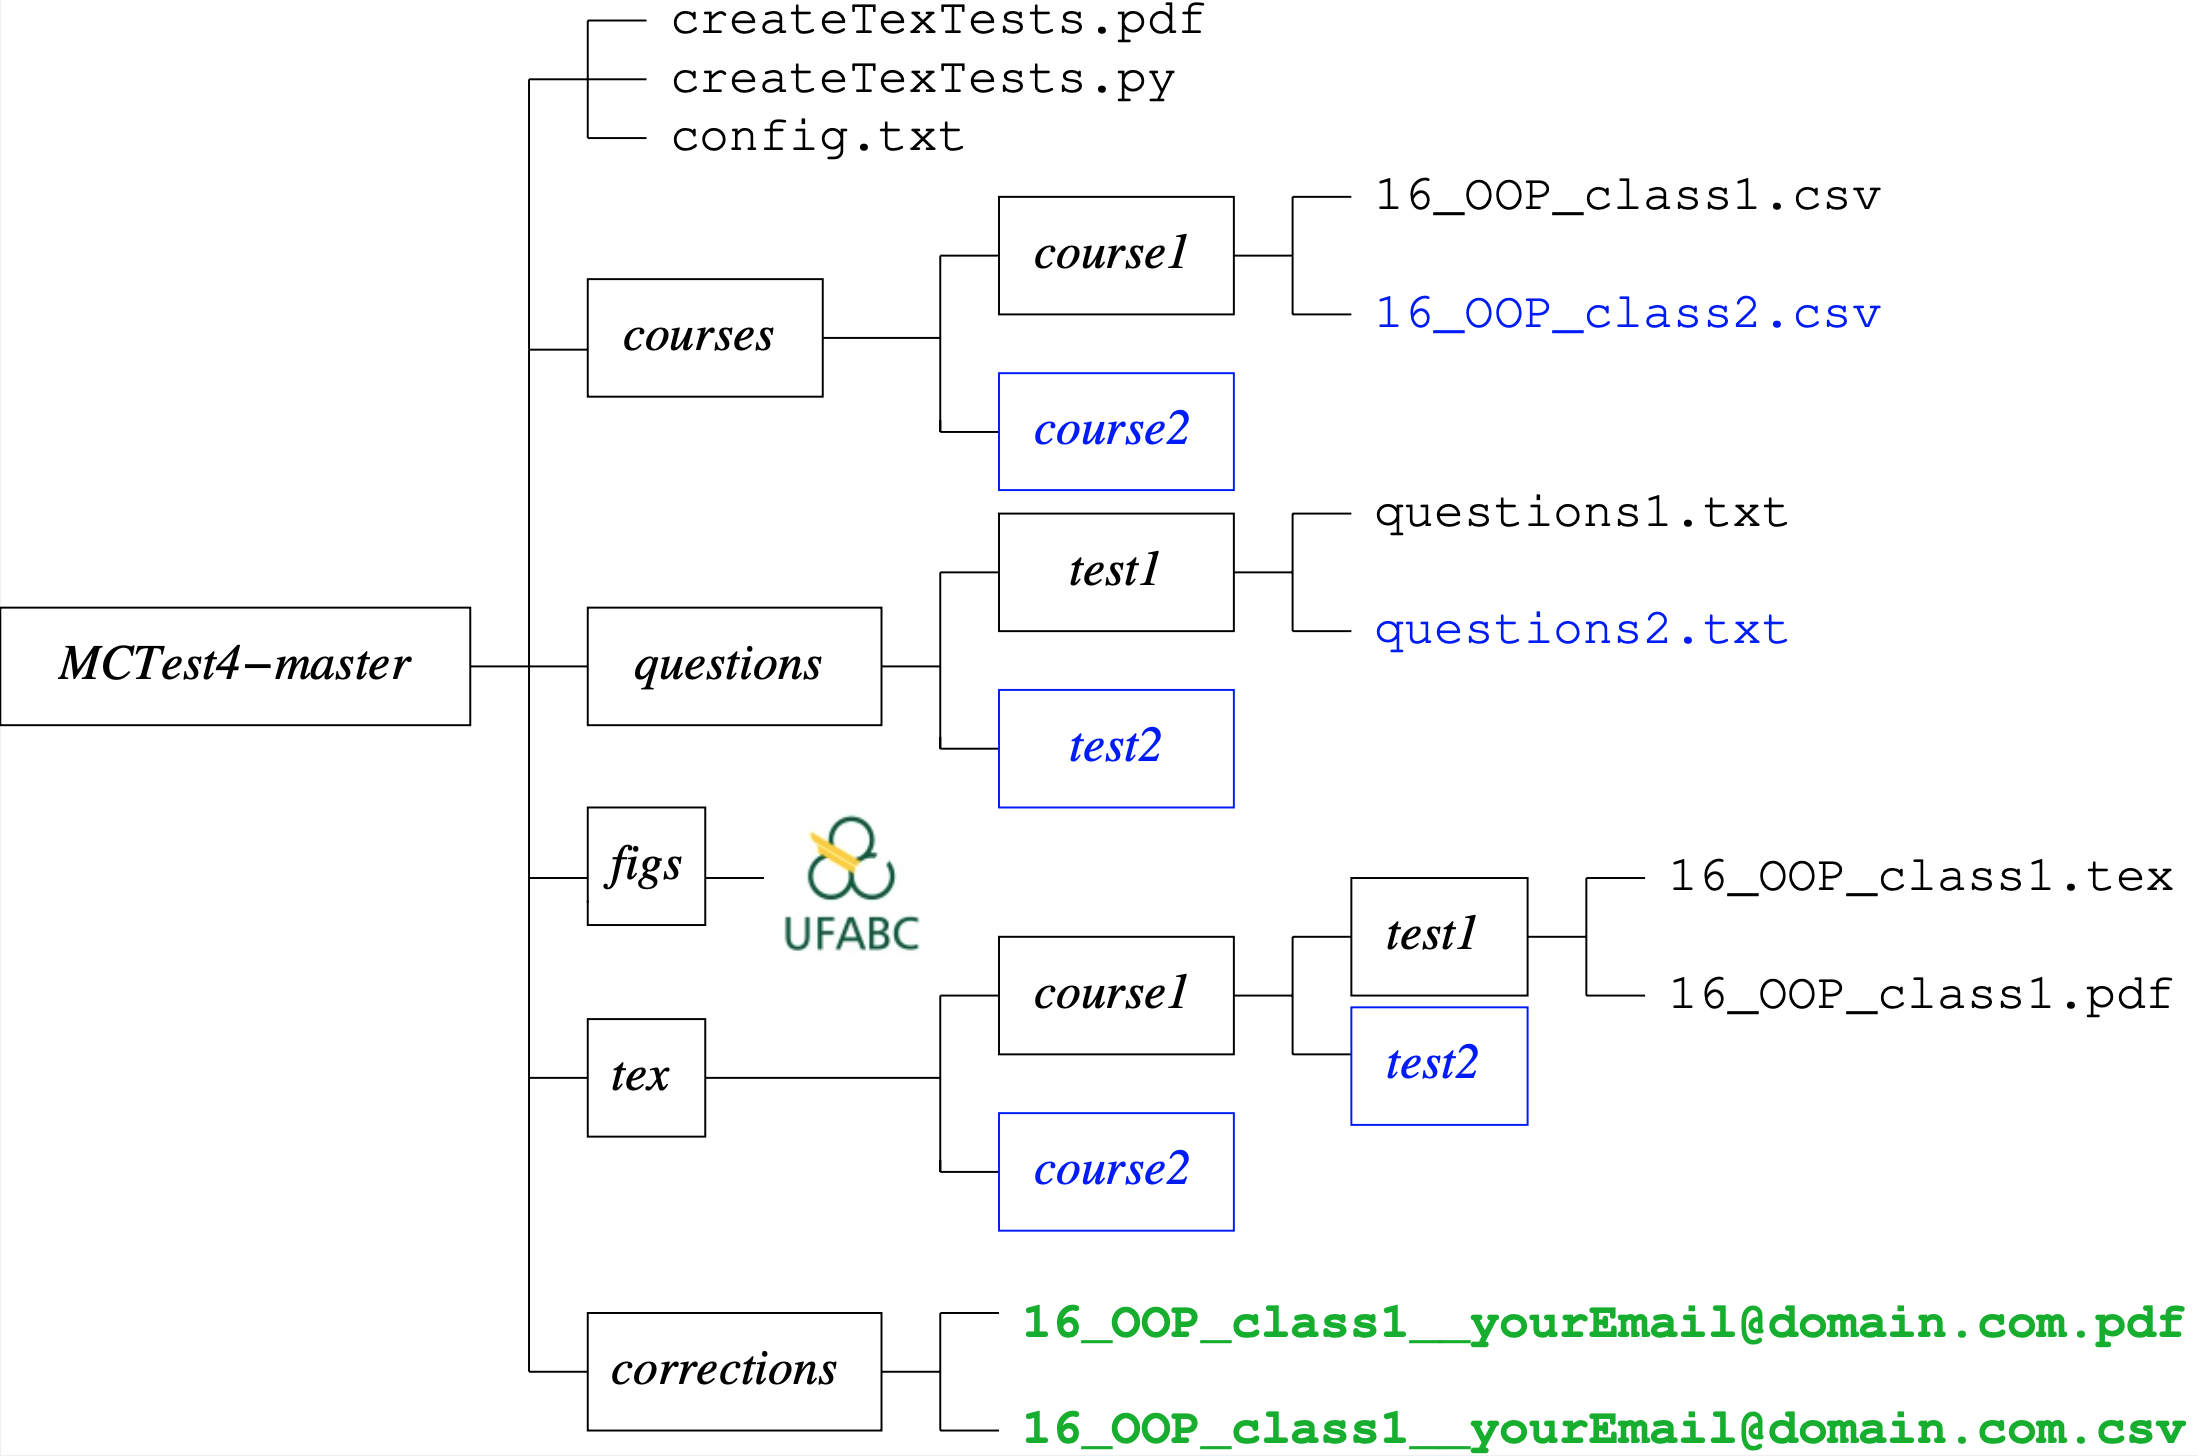
\includegraphics[width=0.85\textwidth]{cap12_mctest4_pastas.png}
\caption{Estrutura de pastas do MCTest-4. \ Fonte: \ \citeonline{2016:Zampirolli.Batista.ea}.}
\label{fig:cap12_mctest4_pastas}
\end{figure}

A pasta \verb|MCTest4-master|, mostrada na Figura \ref{fig:cap12_mctest4_pastas}, contém cinco subpastas, incluindo a pasta \verb|courses|, destinada a armazenar diferentes turmas de uma mesma disciplina ou de disciplinas diferentes. Por exemplo, se você estiver lecionando Programação Orientada a Objetos (POO) e Engenharia de Software (ES) em um semestre de 2016, poderá criar as pastas \verb|course1| e \verb|course2| dentro de \verb|courses| para as turmas de POO e ES, respectivamente. Cada pasta conterá listas de estudantes e seus respectivos IDs em arquivos CSV, como \verb|16_POO_class1.csv| e \verb|16_ES_class2.csv|, seguindo a formatação definida na Seção \ref{sec:professorCriarTurma} -- \nameref{sec:professorCriarTurma}. As questões são armazenadas na pasta \verb|questions| em arquivos TXT, seguindo a mesma estrutura apresentada na Seção \ref{sec:questaoNavegacao} -- \nameref{sec:questaoNavegacao}. A geração de um exame para uma turma específica requer a configuração no arquivo \verb|config.txt|. Para mais detalhes sobre essa estrutura de pastas e arquivos, consulte o artigo de \citeonline{2016:Zampirolli.Batista.ea}.

Os estudantes preenchem os QRs na página inicial do exame, que já contém seus nomes e números de identificação em um código de barras, no caso de exames individuais. Após a conclusão do exame, todas as páginas com os QRs podem ser digitalizadas em um único arquivo PDF, que o software utiliza para realizar a correção automática. As notas finais são armazenadas em um arquivo CSV que contém o ID de cada estudante, seguindo o mesmo estilo apresentado na Seção \ref{sec:CSVcorrecoesQR} - \nameref{sec:CSVcorrecoesQR}.

O programa \verb|createTexTests.py|, apresentado na Figura \ref{fig:cap12_mctest4_pastas}, é responsável por gerar um arquivo GAB contendo os gabaritos das respostas individuais de cada estudante, caso sejam utilizados exames aleatórios. O corretor, por sua vez, lê um arquivo PDF contendo as páginas digitalizadas dos exames e utiliza o arquivo GAB para calcular as notas. As respostas dos estudantes são identificadas através da análise das marcações nas questões. Caso ocorram erros de leitura do código de barras ou das marcações, o corretor sinaliza esses problemas nas notas. O arquivo de notas é gerado em formato CSV.

O MCTest-4 foi elaborado utilizando a linguagem de programação Python e se encontra disponível gratuitamente em \href{https://github.com/fzampirolli/MCTest4}{github.com/fzampirolli/MCTest4}. Professores podem fazer o \textit{download} do código em Python, acompanhado da estrutura de pastas e exemplares de arquivos, para gerar os exames.

Para utilizar o programa, é necessário que o professor instale o Python e as bibliotecas necessárias, como a OpenCV. Uma alternativa é enviar os arquivos GAB e PDF digitalizados para o servidor do MCTest-4 por meio do FTP. Neste servidor, há um \textit{script} que detecta automaticamente esses arquivos e os processa. O arquivo de notas resultante pode ser enviado por e-mail ou baixado do servidor. Todo esse processo é detalhado no artigo de \citeonline{2016:Zampirolli.Batista.ea}.

\subsubsection{Experimentos}

Segundo os autores do artigo, são descritos três experimentos realizados com o MCTest-4. O primeiro experimento foi realizado com uma turma de 66 estudantes da disciplina de Programação Orientada a Objetos. Os exames foram gerados com 10 QMs e uma QT. Os resultados foram satisfatórios, com apenas um erro de leitura. O segundo experimento foi realizado com uma turma de 130 estudantes da disciplina de Processamento de Informação. Os exames foram gerados com 12 QMs e uma QT. Os resultados também foram satisfatórios, sem nenhum erro de leitura. O terceiro experimento foi realizado com 6772 estudantes de escolas públicas do Brasil. Os exames foram gerados com 11 QMs para os estudantes do ensino médio e 13 questões para os estudantes do ensino fundamental. Os resultados foram satisfatórios, com uma taxa de erros de leitura de 1,88\%.

No terceiro experimento, foi utilizado um servidor adquirido com recursos da FAPESP, processo \href{https://bv.fapesp.br/pt/auxilios/28430/modelagem-de-objetos-usando-morfologia-matematica-e-grafos-de-vizinhanca/}{2009/14430–1}, com um microprocessador, \verb|Intel (R) Core (TM) i7|, \verb|CPU X980@3.33GHz| com \verb|12GB| de RAM, sistema operacional Linux Ubuntu 64 bits versão 15.04 e executáveis gerados por Python 2.7.9. Um \textit{script} do MCTest-4 é executado a cada minuto e procura por arquivos com extensão PDF (sem arquivos GAB), para os quais os arquivos CSV correspondentes ainda não foram criados. O corretor automático levou 102 minutos para processar os 6772 exames, ou seja, 0,9 segundos por exame.

Os resultados dos experimentos indicam que o MCTest-4 é uma ferramenta eficaz para a avaliação de estudantes. O programa consegue gerar exames com questões de qualidade e de corrigi-los de forma rápida e precisa. Além disso, o programa é fácil de usar e pode ser personalizado para atender às necessidades específicas de cada professor.

%%%%%%%%%%%%%%%%%%%%%%%%%%%%%%%%%%%%%%%%%%%%%%%%%%%%%%%%%%%%%%%%%%%%%%%%%
\subsection{Artigo comparando as modalidades semipresencial e presencial CS1 com base na utilidade do MCTest-4}\label{sec:experMCTest-4revista}
%%%%%%%%%%%%%%%%%%%%%%%%%%%%%%%%%%%%%%%%%%%%%%%%%%%%%%%%%%%%%%%%%%%%%%%%%

O artigo de \citeonline{2018:Zampirolli.Goya.ea}, publicado na revista \textit{Computer Applications in Engineering Education}, descreve um processo de avaliação desenvolvido para a disciplina de Processamento da Informação (ou Introdução à Programação, IP, ou também CS1) oferecido pela Universidade Federal do ABC. O estudo compara a modalidade presencial (IP-FF -- \textit{face-to-face}) e a modalidade semipresencial \textit{blended learning} (IP-BL), na qual apenas as avaliações são realizadas presencialmente. 

\subsubsection{Método}

O processo de avaliação foi desenvolvido a partir da identificação de problemas no processo de avaliação de IP-FF. Os problemas identificados foram: Avaliação de critérios diferentes entre professores; falta de uniformidade na formatação dos exames; dificuldade de calcular a nota final do estudante.

Para resolver esses problemas, o processo de avaliação proposto utiliza: um banco de questões com diferentes níveis de dificuldade; um sistema para gerar exames únicos para cada estudante; um sistema para corrigir os exames de forma semi-automática.

\subsubsection{Experimentos}

Os experimentos foram conduzidos em 10 turmas da disciplina IP-BL e demonstraram que o processo de avaliação conseguiu padronizar os critérios de avaliação, aprimorar a formatação dos exames e simplificar o cálculo da nota final. Os exames foram elaborados utilizando adaptações no software MCTest-4.G, contendo três QTs em cada exame. Para aumentar a diversidade, as questões foram replicadas manualmente com modificações em alguns parâmetros.

Foram criados \textit{scripts} em Python para auxiliar nas avaliações da disciplina. Essas ferramentas automatizadas incluem a geração automática de exames individuais, a organização dos exames digitalizados por questão e estudante, a compilação do código submetido pelos estudantes e o envio automático de e-mails com as notas e os erros apontados pelos professores. Todos esses \textit{scripts} foram adaptados e incorporados na versão web mais recente, MCTest-5.

A primeira avaliação da disciplina foi realizada em formato impresso, na qual os estudantes tinham que resolver três EPs. Uma das questões envolvia o uso de teste de mesa, conforme ilustrado na Figura \ref{fig:cap04_figQuestaoAtualizaPDF4}. Um exemplo de exame utilizado para essa primeira avaliação, em que cada questão ocupava uma folha frente e verso, é mostrado na Figura \ref{fig:cap12_mctest4_folha}. As resoluções dos estudantes eram digitalizadas e enviadas aos professores, sendo que cada professor corrigia uma única questão de todos os estudantes da disciplina na modalidade IP-BL.

Na segunda avaliação, os estudantes também tinham que resolver três EPs, mas desta vez elas foram enviadas por meio da plataforma AVA (Ambiente Virtual de Aprendizagem) \href{http://tidia4.ufabc.edu.br/portal}{tidia4.ufabc.edu.br}. Todos os códigos submetidos pelos estudantes foram salvos em um computador e executados automaticamente para verificar possíveis erros. Os professores deveriam atribuir um conceito a cada arquivo de código.

Essas correções unificadas ocorreram nos anos de 2016.3, 2017.1 e 2017.2, com um total de 235, 185 e 161 estudantes, respectivamente. A UFABC utiliza três períodos letivos por ano.

Esses aquivos de códigos dos estudantes foram também utilizados como \textit{dataset} para o artigo de \citeonline{2019:Souza.Zampirolli.ea}, que apresenta um método para validar as notas atribuídas por professores aos EPs de estudantes em IP-BL. Foi utilizado um modelo de rede neural convolucional treinado com códigos fonte de estudantes avaliados por diferentes professores. Os códigos foram pré-processados e convertidos em representações \textit{embedding}, utilizadas como entrada para a rede neural. O modelo obteve uma precisão média de 74,9\% na classificação das notas dos exercícios. Essa abordagem pode ajudar a detectar possíveis erros no processo de avaliação realizado pelos professores.

\begin{figure}[!ht]
\centering
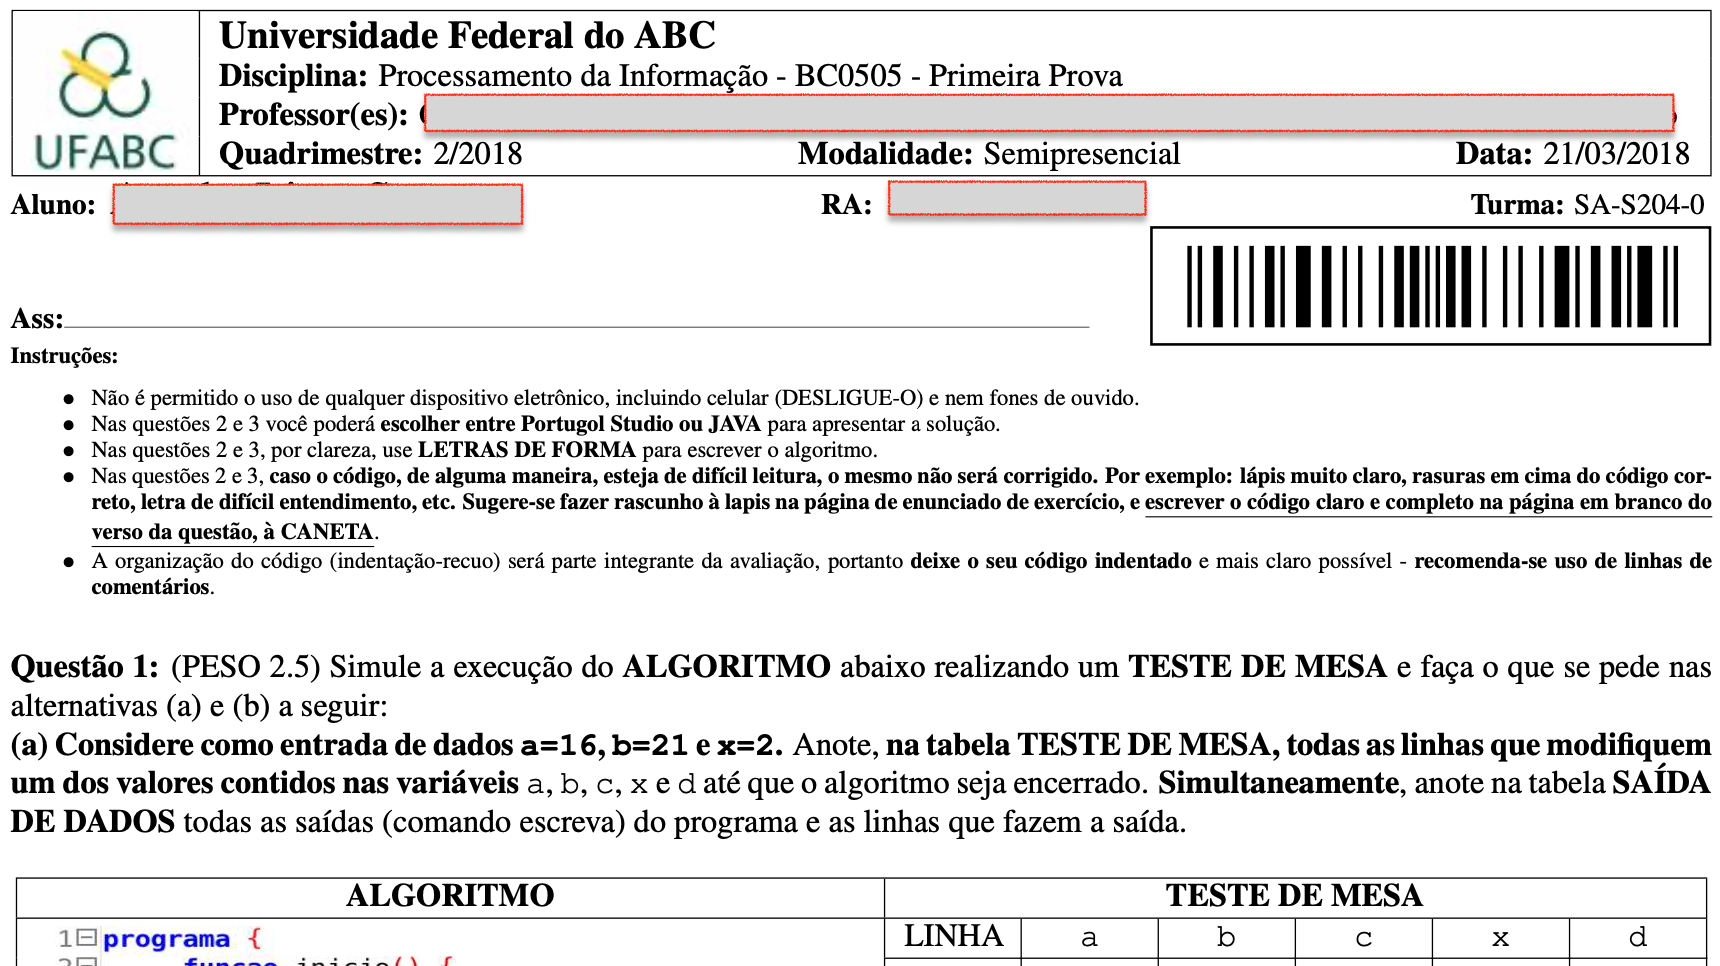
\includegraphics[width=0.9\textwidth]{cap12_mctest4_folha.png}
\caption{Recorte de um exame gerado com MCTest-4.G.}
\label{fig:cap12_mctest4_folha}
\end{figure}

Os resultados mostraram a redução da dispersão nas notas após a implementação do processo de avaliação unificado. No entanto, ainda é preciso enfrentar desafios como a resistência dos professores em adotar critérios unificados e a incorporação de ferramentas de correção automática no AVA. O artigo ressalta a importância de atividades de motivação e acompanhamento dos estudantes para melhorar os índices de aprovação na disciplina.

%%%%%%%%%%%%%%%%%%%%%%%%%%%%%%%%%%%%%%%%%%%%%%%%%%%%%%%%%%%%%%%%%%%%%%%%%
\subsection{Artigo definindo a parametrização do MCTest após a versão 4}\label{sec:definindoParametrizacao}
%%%%%%%%%%%%%%%%%%%%%%%%%%%%%%%%%%%%%%%%%%%%%%%%%%%%%%%%%%%%%%%%%%%%%%%%%

Todo o conteúdo apresentado no Capítulo \ref{ch:questoesCodigoMCTest} -- \nameref{ch:questoesCodigoMCTest}, exceto a seção referente ao VPL, foi originalmente publicado no artigo de \citeonline{2019:Teubl.Batista.ea}. Em resumo, para criar questões paramétricas no MCTest-4, são necessários dois delimitadores especiais: \verb|[[code:...]]| e \verb|[[def:...]]|. O primeiro deve ser colocado no enunciado da questão ou nas alternativas e define instruções em Python ou variáveis a serem usadas na geração do exame de cada estudante. Já o segundo deve ser definido no final do enunciado e deve conter os possíveis valores para as variáveis aplicadas anteriormente.

Esse artigo apresenta duas questões paramétricas utilizando arquivos TXT, conforme apresentado na Seção \ref{sec:questaoNavegacao} - \nameref{sec:questaoNavegacao}, reproduzidas a seguir. Lembrando que a contribuição desse artigo criou questões paramétricas e na época da escrita do artigo, a versão web ainda não estava disponível. A seguir, são apresentadas essas questões, porém, na versão web do MCTest.

\subsubsection{Movimento Retilíneo Uniforme com a biblioteca \texttt{symbols}}

O Código \ref{lst:questaoQM_MRU} implementa um algoritmo para calcular a variável tempo (\verb|t|) em um problema de Movimento Retilíneo Uniforme (MRU), dado a posição inicial (\verb|s0|), a velocidade (\verb|v|) e a posição final (\verb|s|) do corpo.
O método \verb|algorithm(a)| recebe como entrada uma lista contendo três valores inteiros: a posição inicial (\verb|s0|), a velocidade (\verb|v|) e a posição final (\verb|s|), nessa ordem.
Na primeira linha do método, são importados os módulos \verb|symbols| e \verb|solve| da biblioteca SymPy (\href{https://docs.sympy.org}{docs.sympy.org}), que permite criar símbolos matemáticos para serem usados em cálculos simbólicos e também resolver uma equação, respectivamente.
São definidos os símbolos \verb|s| e \verb|t| utilizando o método \verb|symbols|, e a posição \verb|s| é calculada como a soma da posição inicial \verb|s0| com a velocidade \verb|v| multiplicada pelo tempo \verb|t|.
Por fim, o método \verb|solve| é utilizado para resolver a equação \verb|s-a2=0| em relação à variável \verb|t|. O resultado é armazenado na variável \verb|r| como um número decimal (do tipo \verb|float|) e retornado pelo método \verb|algorithm(a)| como o tempo necessário para o objeto percorrer a distância entre as posições \verb|s0| e \verb|s| com velocidade \verb|v| em MRU. Um exemplo de saída desta questão pode ser visualizado na Figura \ref{fig:cap12_questaoQM_MRUPDF}.

\begin{listing}[!ht]
\begin{myboxCode}{corCodigo}{\textbf{Questão: }}\vspace{3mm}
\hrule
\begin{minted}[xleftmargin=20pt,linenos=true]{python}
Um automóvel percorre uma estrada com função horária \( s=[[code:a0]] + 
[[code:a1]]t \), onde \(s\) é dado em quilômetros e \(t\) em horas. 
O automóvel passa pelo km [[code:a2]] após:

[[def:
def generate_numbers():
    """ Gera três números aleatórios e retorna-os como uma lista. """
    import random
    global a0, a1, a2 # necessário declarar como global para utilizar no enunciado
    a0 = random.randrange(-6, 12, 1)  # s0 - posição inicial
    a1 = random.randrange(3, 8, 1)    # v  - velocidade
    a2 = random.randrange(3, 8, 1)    # s  - posição final
    return [a0, a1, a2]

def algorithm(a):
    """ Executa um algoritmo matemático utilizando os valores passados como 
    parâmetro. Retorna o resultado do algoritmo. """
    from sympy import symbols, solve
    a0, a1, a2 = a  # s0, v, s
    s, t = symbols('s,t')
    s = a0 + a1 * t

    r = float(solve(s - a2, t)[0])
    return r

# Gera os números aleatórios
numbers = generate_numbers()

# Executa o algoritmo utilizando os números gerados
correctAnswer = algorithm(numbers)
# [[code:f"{correctAnswer:.2f}"]]

# Opções de respostas erradas com base no resultado do algoritmo
# [[code:f"{correctAnswer+1.2:.2f}"]]
# [[code:f"{correctAnswer+4.8:.2f}"]]
# [[code:f"{correctAnswer-0.9:.2f}"]]
]]
\end{minted}
\end{myboxCode}
\caption{Exemplo de QM paramétrica para calcular MRU.}
\label{lst:questaoQM_MRU}
\end{listing}

\begin{figure}[!ht]
  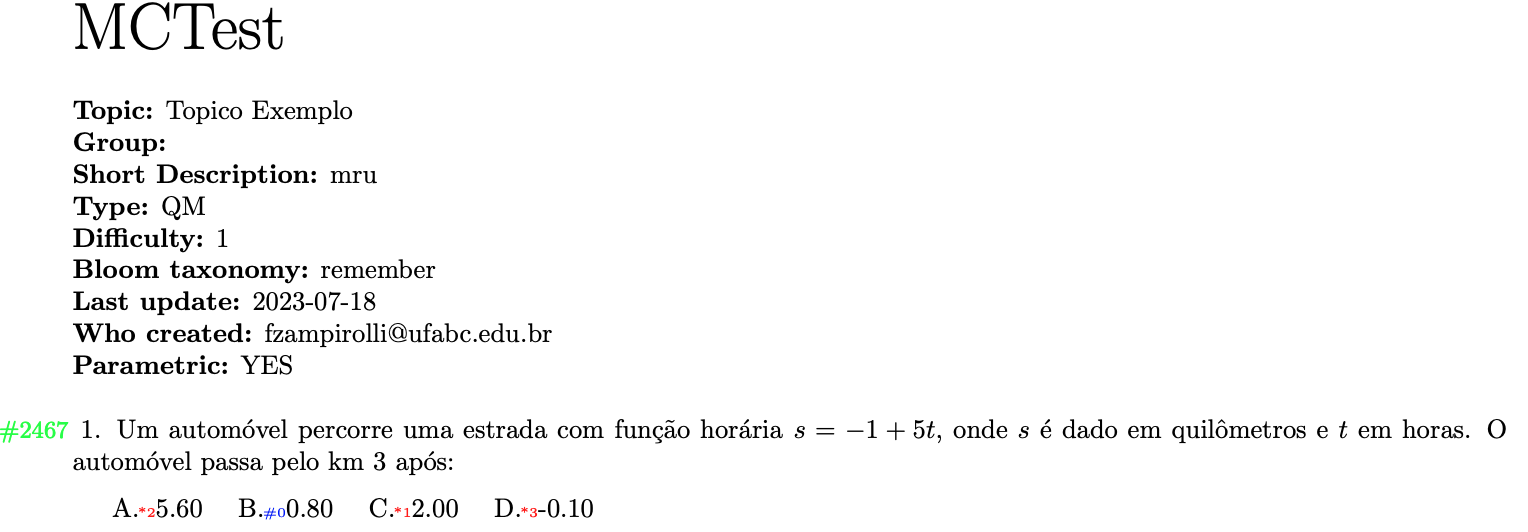
\includegraphics[width=0.9\textwidth]{cap12_questaoQM_MRUPDF.png}
  \caption{Recorte do PDF gerado para a questão de MRU do Código \ref{lst:questaoQM_MRU}.}
  \label{fig:cap12_questaoQM_MRUPDF}
\end{figure}

\begin{mybox}{corCopia}{\textbf{Atenção:\\\vspace{-3mm}\hrule\vspace{1mm}}}
\begin{enumerate}
\item  Toda variável declarada em um método e utilizada no enunciado da questão deve ser definida como global, como pode ser visto na linha 9 do Código \ref{lst:questaoQM_MRU};
\item As importações de bibliotecas também devem ser realizadas nos métodos, como podem ser vistos nas linhas 8 e 18.
\end{enumerate}
\end{mybox}


\subsubsection{Criação de Matriz}

A questão a seguir é uma adaptação daquela apresentada na Seção \ref{sec:questaoNavegacao} -- \nameref{sec:questaoNavegacao}, porém, agora é parametrizada com as dimensões da matriz e os elementos atribuídos. O Código \ref{lst:questaoQM_criaMatriz} é responsável por criar uma matriz  \(M\) com dimensões \( [[\text{code:Linhas}]] \times [[\text{code:Colunas}]] \). Cada elemento da matriz é calculado utilizando a fórmula \( (i,j) = ((((i+1) \times [[\text{code:a2}]]) + ((j+1) \times [[\text{code:a3}]])) \mod{100}) \), em que \(i\) representa as linhas e \(j\) representa as colunas da matriz.
%
Na prática, o código gera aleatoriamente o número de linhas e colunas da matriz, num intervalo específico, assim como os valores de \(a2\) e \(a3\), escolhidos aleatoriamente entre as opções [7, 13, 19] e [11, 17, 23], respectivamente.
%
A matriz é inicializada com zeros e, em seguida, preenchida utilizando dois laços aninhados. Cada elemento \(M[i,j]\) recebe o resultado do cálculo mencionado anteriormente.
%
Por fim, a variável global \verb|correctAnswer| é definida como a soma de todos os elementos da matriz \(M\). Um exemplo de saída desta questão pode ser visualizado na Figura \ref{fig:cap12_questaoQM_criaMatrizPDF}.


\begin{listing}[!ht]
\begin{myboxCode}{corCodigo}{\textbf{Questão: } }\vspace{3mm}
\hrule
\begin{minted}[xleftmargin=20pt,linenos=true]{python}
Criar uma matriz \( [[code:Linhas]] \times [[code:Colunas]] \) com elementos 
\( (i,j) = ((((i+1) * [[code:a2]]) + ( ( j+1) * [[code:a3]])) \mod{100}) \). 
Calcular a soma dos elementos desta matriz. Os índices \(i\) são as linhas
e \(j\) as colunas iniciadas com o valor \(0\).

[[def:
import numpy as np, random

# Gerar número aleatório de linhas e colunas
Linhas = np.random.randint(4, 8)
Colunas = np.random.randint(4, 8)

# Escolher valores aleatórios para a2 e a3
a2 = random.choice([7, 13, 19])
a3 = random.choice([11, 17, 23])

# Inicializar matriz com zeros
M = np.zeros((Linhas, Colunas), dtype=int)

# Preencher a matriz com os cálculos
for i in range(Linhas):
    for j in range(Colunas):
        M[i, j] = (((i+1) * a2) + ((j+1) * a3)) % 100

# Calcular a soma dos elementos da matriz
correctAnswer = np.sum(M)

# Incluir nas alternativas da questão: 
# [[code:correctAnswer]] % primeira alternativa (sempre) correta
# [[code:createWrongAnswers([3,10])]] % cria 3 alter. erradas +/- 10
]]
\end{minted}
\end{myboxCode}
\caption{Exemplo de QM paramétrica para criar uma matriz.}
\label{lst:questaoQM_criaMatriz}
\end{listing}

\begin{figure}[!ht]
  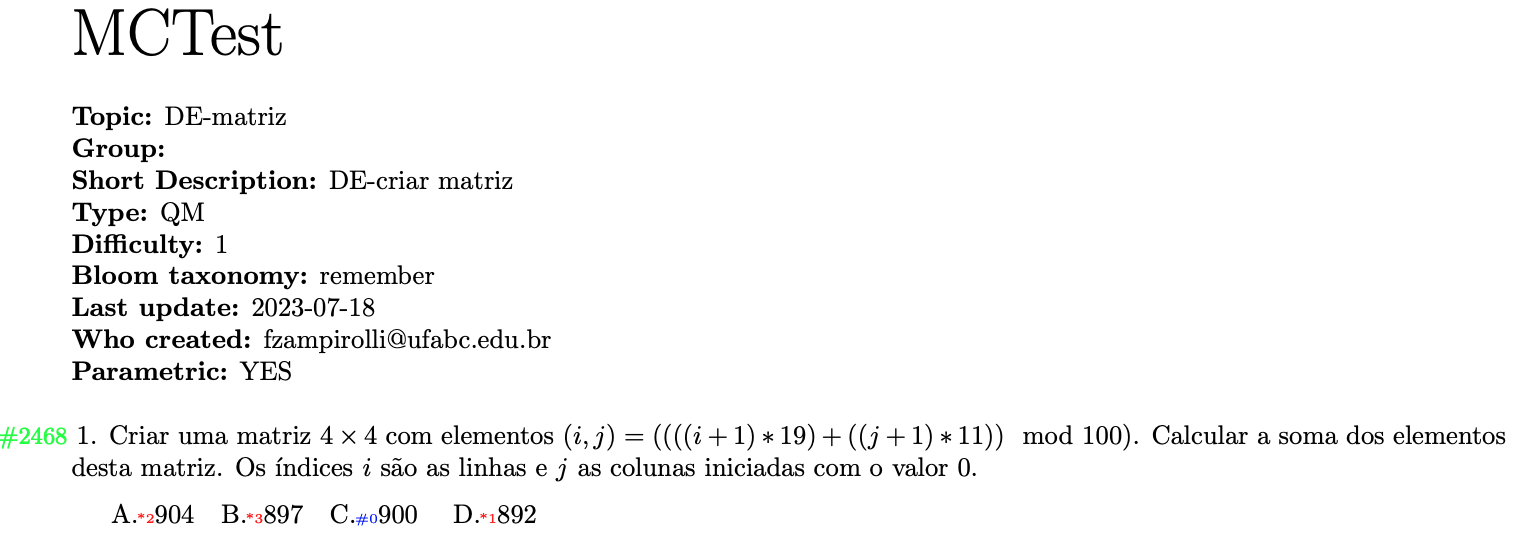
\includegraphics[width=0.9\textwidth]{cap12_questaoQM_criaMatrizPDF.png}
  \caption{Recorte do PDF gerado para a questão para criar uma matriz do Código \ref{lst:questaoQM_criaMatriz}.}
  \label{fig:cap12_questaoQM_criaMatrizPDF}
\end{figure}

\subsubsection{Experimentos}

O método proposto para gerar questões paramétricas foi aplicado na disciplina de Processamento da Informação (ou Introdução à Programação, IP, ou também CS1) no segundo trimestre de 2018, com um total de 167 estudantes matriculados. A disciplina foi oferecida em um formato semipresencial, com aulas presenciais ocorrendo em quatro momentos ao longo do semestre: na abertura, no primeiro exame, no projeto e no segundo exame.

A disciplina CS1 faz parte de um programa de bacharelado interdisciplinar oferecido pela universidade, e os estudantes que a cursam têm origens diversas. O método se baseia no software MCTest-4, que permite gerar várias versões diferentes da mesma questão sem repetições. Para cada estudante, foram geradas três questões de dificuldades diferentes (fácil, média e difícil), porém com a preocupação de não deixar uma variação de exame mais difícil que a outra.

Os resultados dos experimentos mostraram que o método proposto foi eficaz na geração de questões paramétricas para exames impressos. Além disso, o uso do MCTest-4 facilitou a correção automática dos exames com QMs.


%%%%%%%%%%%%%%%%%%%%%%%%%%%%%%%%%%%%%%%%%%%%%%%%%%%%%%%%%%%%%%%%%%%%%%%%%
%%%%%%%%%%%%%%%%%%%%%%%%%%%%%%%%%%%%%%%%%%%%%%%%%%%%%%%%%%%%%%%%%%%%%%%%%
\section{MCTest-5: a versão web}
%%%%%%%%%%%%%%%%%%%%%%%%%%%%%%%%%%%%%%%%%%%%%%%%%%%%%%%%%%%%%%%%%%%%%%%%%
%%%%%%%%%%%%%%%%%%%%%%%%%%%%%%%%%%%%%%%%%%%%%%%%%%%%%%%%%%%%%%%%%%%%%%%%%

A partir deste ponto, todas as publicações foram conduzidas utilizando a versão web MCTest-5, que será mencionada simplesmente como MCTest. Esta versão possibilitou que os docentes empregassem o MCTest sem a necessidade de instalações locais em seus dispositivos, resultando em notável simplificação tanto na criação como na avaliação de exames, além da viabilização do compartilhamento de questões. A seguir, serão apresentados os artigos diretamente vinculados a esta edição \textit{online}, corroborando sua eficácia e usabilidade, porém, ainda sem a integração do VPL no Moodle.

%%%%%%%%%%%%%%%%%%%%%%%%%%%%%%%%%%%%%%%%%%%%%%%%%%%%%%%%%%%%%%%%%%%%%%%%%
\subsection{Artigo apresentando a primeira versão web do MCTest}\label{sec:MTest-5_web}
%%%%%%%%%%%%%%%%%%%%%%%%%%%%%%%%%%%%%%%%%%%%%%%%%%%%%%%%%%%%%%%%%%%%%%%%%

O artigo de \citeonline{2019:Zampirolli.Teubl.ea} apresentou a primeira versão web do MCTest para geração e correção de questões parametrizadas, aplicável a diversas disciplinas e instituições educacionais. O método desenvolvido permite criar exames com variações nos textos, mantendo o mesmo conteúdo e nível de dificuldade. Para facilitar o processo, foram desenvolvidas interfaces gráficas que permitem coletar informações sobre instituições, cursos, disciplinas, tópicos, turmas, exames e questões.

O artigo apresenta as primeiras versões dessas interfaces gráficas, com ênfase na versão mais recente discutida nos Capítulos \ref{ch:visaoGeral} - \nameref{ch:visaoGeral}, \ref{ch:questoesClassicasMCTest} - \nameref{ch:questoesClassicasMCTest} e \ref{ch:questoesCodigoMCTest} - \nameref{ch:questoesCodigoMCTest}. Os resultados detalhados da implementação desse método são apresentados neste Capítulo \ref{ch:questoesCodigoMCTest}.

O processo de geração de questões parametrizadas utiliza principalmente a linguagem de programação Python, com alguns elementos de \LaTeX{} presentes no enunciado das questões. Os resultados obtidos demonstram a eficiência do sistema, mesmo em sua primeira versão, que foi implementada em páginas web escritas em Django. O sistema é gratuito e oferece aos professores a capacidade de gerar e corrigir exames automaticamente para centenas ou milhares de estudantes.

A seguir, serão apresentados exemplos das questões paramétricas discutidas neste artigo.

\subsubsection{Equações paramétricas com equação e figura utilizando a biblioteca \texttt{sympy}}\label{sec:equacao_sympy_figura}

A seguir é apresentado um exemplo de questão paramétrica que inclui uma equação matemática e uma figura. Neste caso, a equação envolve funções seno, cosseno e integração.

O Código \ref{lst:questaoQM_equacaoFigura} primeiro importa as bibliotecas \verb|sympy| e \verb|random|. A biblioteca SymPy, disponível em \href{https://docs.sympy.org}{docs.sympy.org}, fornece funções para trabalhar com expressões simbólicas. O código então gera três números aleatórios, \verb|a1|, \verb|a2| e \verb|a3|, escolhidos entre 3 e 6, 2 e 4, e 1 e 3, respectivamente. Esses números serão usados para definir os parâmetros da função. O código então define a variável simbólica \verb|x| e a função \verb|f|. A função \verb|f| é uma combinação de funções seno e cosseno com os parâmetros \verb|a1|, \verb|a2| e \verb|a3|. O código então desenha o gráfico da função \verb|f| no intervalo de -5 a 5. A imagem do gráfico é salva no arquivo \verb|./tmp/imgs180days/fz_figIntegral_01_{a1}_{a2}_{a3}_{h}.png|. O código então calcula a integral da função \verb|f|. A integral é calculada usando a função \verb|integrate| da biblioteca SymPy. O código então converte a integral para notação \LaTeX{}. Por fim, o código imprime as seguintes expressões em notação \LaTeX{}: a integral da função \verb|f|, a resposta correta à pergunta e três respostas incorretas.

\begin{mybox}{corCopia}{\textbf{Atenção:\\\vspace{-3mm}\hrule\vspace{1mm}}}
\begin{enumerate}
\item A inclusão de imagens em arquivo \LaTeX{} pode tornar a compilação para gerar o PDF muito lenta;
\item Uma sugestão é salvar as imagens no servidor do MCTest, disponível no seguinte \textit{link}: \url{http://mctest.ufabc.edu.br:8000/tmp/imgs180days/}. Esse servidor antes do \verb|/tmp/| deve ser alterado a cada implantação do MCTest. O professor pode incluir um \textit{link} para essa imagem no enunciado da questão, permitindo que os estudantes acessem durante a realização do exame.
\item Todos os arquivos temporários são eliminados automaticamente do servidor após 180 dias; contudo, essa configuração pode ser ajustada;
\item É fundamental incluir os parâmetros no nome do arquivo da imagem caso a questão seja paramétrica e a imagem varie conforme esses parâmetros. Isso pode ser feito como demonstrado nas linhas 22 a 29 do Código \ref{lst:questaoQM_equacaoFigura}, em que uma \textit{string} contendo os valores dos parâmetros é usada para gerar um objeto \textit{hash}, convertido em uma \textit{string} legível e adicionado ao nome do arquivo de imagem. Dessa forma, cada imagem gerada terá um nome único, garantindo que não haja conflitos entre elas.
\end{enumerate}
\end{mybox}

Merece uma explicação especial o nome do arquivo em que será salva a imagem gerada. Esse arquivo deve ser único, minimizando a chance de criar um arquivo com o mesmo nome de outro que já existe. Para garantir isso, é utilizada a biblioteca \verb|hashlib| na linha 23 do Código \ref{lst:questaoQM_equacaoFigura}. Em seguida, o código cria uma \textit{string} \verb|s| que contém os valores dos parâmetros \verb|a1|, \verb|a2| e \verb|a3|. Essa \textit{string} é usada para criar um objeto \textit{hash}, que será usado para gerar um nome único para o arquivo de imagem. Depois, o objeto \textit{hash} é convertido em uma \textit{string} legível e adicionado ao nome do arquivo de imagem. Esse nome é composto pelo prefixo \verb|./tmp/imgs180days/fz_figIntegral_01_|, seguido pelos valores dos parâmetros \verb|a1|, \verb|a2| e \verb|a3| e pelo \textit{hash} gerado anteriormente. Por fim, o sufixo \verb|.png| indica que a imagem será salva em formato PNG. Dessa forma, é possível gerar imagens únicas para diferentes valores dos parâmetros.

\begin{listing}[!ht]
\begin{myboxCode}{corCodigo}{\textbf{Questão: }}\vspace{3mm}
\hrule
\begin{minted}[xleftmargin=20pt,linenos=true]{python}
A integral da função  \([[code:a0]]\) tem seu gráfico representado abaixo. 
Calcule o valor da integral e marque a alternativa correta.

\begin{figure}[ht!]
\centering \includegraphics[scale=0.7]{[[code:figura]]} 
\centerline{Figura da integral}
\end{figure}

[[def:
from sympy import symbols, sin, cos, plot, latex, Integral, integrate
import random

# Geração dos parâmetros aleatórios
a1 = random.randrange(3, 6, 1)
a2 = random.randrange(2, 4, 1)
a3 = random.randrange(1, 3, 1)

# Definição da variável simbólica e da função
x = symbols('x')
f = a1*sin(a2*x) - a3*cos(x)

# Plotagem da função
import hashlib
s =str([a1,a2,a3]) 
h = hashlib.md5(s.encode()) # create hash - arquivo único
h = str(h.hexdigest())
p = plot(f, (x, -5, 5), show=False)
figura = f'./tmp/imgs180days/fz_figIntegral_01_{a1}_{a2}_{a3}_{h}.png'
p.save(figura)

# Cálculo da integral e conversão para notação LaTeX
a0 = latex(Integral(f, x))
correctAnswer = latex(integrate(f, x))
error1 = latex(integrate(f + x, x))
error2 = latex(integrate(f - x, x))
error3 = latex(integrate(x**5 + x + 1, x))
# nas alternativas: \([[code:correctAnswer]]\); \([[code:error1]]\); ...
]]
\end{minted}
\end{myboxCode}
\caption{Questão paramétrica com equação e figura.}
\label{lst:questaoQM_equacaoFigura}
\end{listing}

\begin{figure}[!ht]
  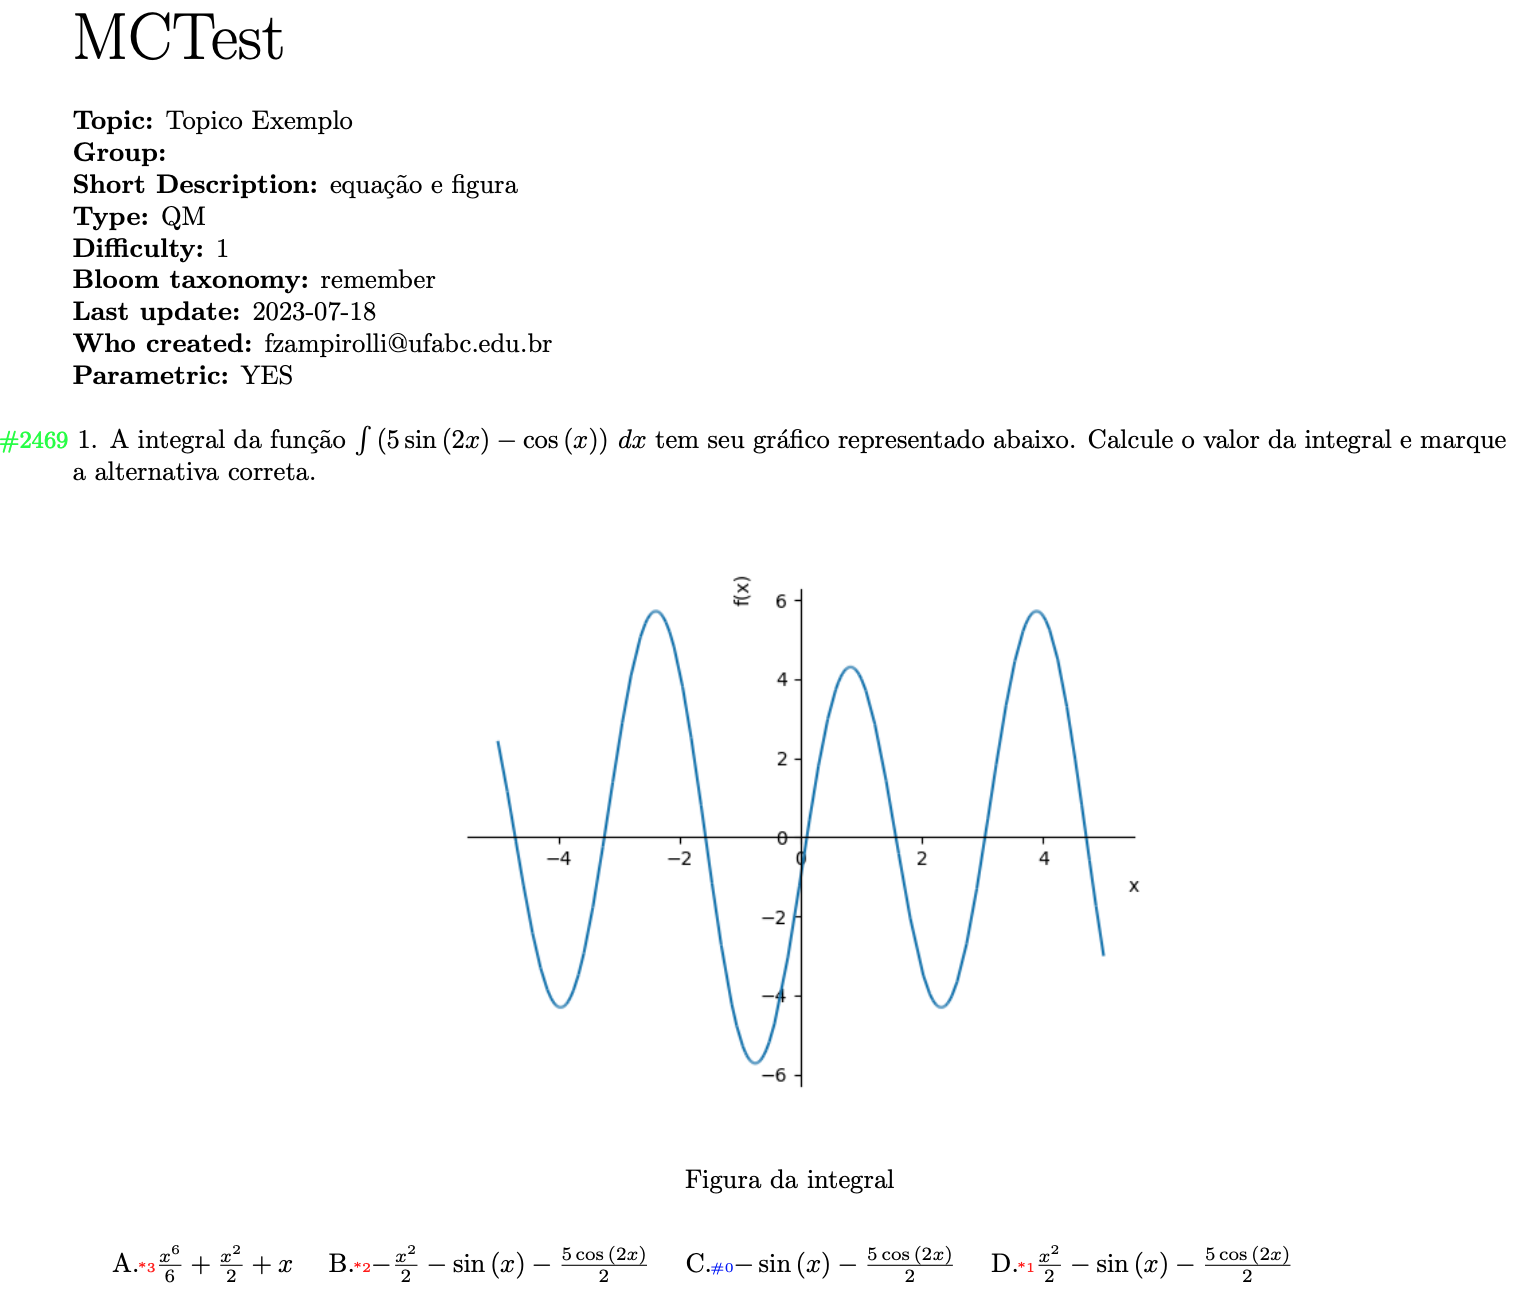
\includegraphics[width=0.9\textwidth]{cap12_questaoQM_equacaoFiguraPDF.png}
  \caption{Recorte do PDF gerado para a questão paramétrica com equação e figura referente ao Código \ref{lst:questaoQM_equacaoFigura}.}
  \label{fig:cap12_questaoQM_equacaoFiguraPDF}
\end{figure}

\begin{mybox}{corCopia}{\textbf{Atenção:\\\vspace{-3mm}\hrule\vspace{3mm}}}
A principal dificuldade ao lidar com questões paramétricas usando a biblioteca SymPy é definir corretamente o intervalo das variáveis aleatórias e também as respostas incorretas das alternativas, sem gerar soluções inexistentes.
\end{mybox}

\subsubsection{Questão paramétrica com grafo e figura}\label{sec:grafo_figura}

A questão paramétrica  apresentada no \ Código \ref{lst:questaoQM_grafo} \ cria o grafo \  \(G = (V, E)\), \ \ em que \ \(V = {n_1, n_2, \cdots, n_p}\) é um conjunto de nós (ou vértices) e \(E\) é um conjunto de arestas (ou arcos), sendo que cada \(e \in E\) é dado por \(e = (n_i, n_j)\) para \(n_i, n_j \in V\). As arestas podem ter peso e o exemplo resolve o problema de encontrar o caminho de peso mínimo. Um caminho é uma sequência de vértices adjacentes, que determina uma sequência de arestas, e o peso do caminho é calculado somando os pesos de suas arestas.

Para gerar a imagem apresentada na Figura \ref{fig:cap12_questaoQM_grafoPDF}, será utilizado o método \verb|draw| da biblioteca NetworkX (\href{https://networkx.org/}{networkx.org}) em conjunto com a biblioteca Matplotlib (\href{https://matplotlib.org/}{matplotlib.org}). No entanto, é importante notar que o código precisa ser modificado para tratar o caso em que existem dois ou mais caminhos mínimos com o mesmo peso. Uma possível solução seria modificar o código para descartar os pesos gerados nas linhas 16 e 17 quando existirem dois caminhos mínimos com o mesmo peso. Essa modificação é análoga à condição de aceitar apenas caminhos com pelo menos 5 vértices, verificada nas linhas 21 e 22. Dessa forma, o código garantiria que apenas um caminho mínimo seria considerado na geração da imagem, o que é necessário para garantir que a QM com alternativas definidas nas linhas 30 e 31 tenha apenas uma correta.



\begin{listing}[!ht]
\begin{myboxCode}{corCodigo}{\textbf{Questão: } }\vspace{3mm}
\hrule
\begin{minted}[xleftmargin=20pt,linenos=true]{python}
Qual é o caminho de Dijkstra neste grafo, entre os nós \(a\) e \(e\), com os 
seguintes pesos \\ \verb|[[code:grafo]]|?

\begin{figure}[!h] 
\centering\includegraphics[scale=0.7]{[[code:pathGrafico]]}
\end{figure} 

[[def:
import matplotlib.pyplot as plt, networkx as nx
from itertools import permutations

while True:
  plt.clf()
  G = nx.Graph() # Definição do grafo
  w1,w2,w3,w4,w5,w6,w7 =  random.sample(range(1,10), 7)
  edges=[('a','b',w1),('b','c',w2),('a','c',w3),('c','d',w4),
   ('b','d',w5),('d','e',w6),('e','c',w7)]
  G.add_weighted_edges_from(edges)
  grafo = str(edges)

  v = nx.dijkstra_path(G, 'a', 'e') # Cálculo do caminho mínimo
  if len(v)<5: continue # aceita pelo menos 5 nós

  perm_list = [] # criar permutações
  for perm in permutations(v):
    if perm[0] == v[0] and perm[-1] == v[-1]:
      perm_list.append(perm)
  break

correctAnswer = str(perm_list[0])
error1,error2,error3 = str(perm_list[1]), str(perm_list[2]), str(perm_list[3])
# nas alternativas: \verb|[[code:correctAnswer]]|\\ ; \verb|[[code:error1]]|\\ ...

pos = nx.spring_layout(G) # Plotagem do grafo
nx.draw(G, pos=pos)
nx.draw_networkx_labels(G, pos=pos)
nx.draw_networkx_edge_labels(G, pos=pos)

import hashlib # Salvando a figura
s =str(edges) 
h = hashlib.md5(s.encode()) # create hash - arquivo único
pathGrafico = 'figGrafo(' + str(h.hexdigest()) + ')' 
plt.savefig(pathGrafico)
]]
\end{minted}
\end{myboxCode}
\caption{QM paramétrica com grafo e figura.}
\label{lst:questaoQM_grafo}
\end{listing}

\begin{figure}[!ht]
  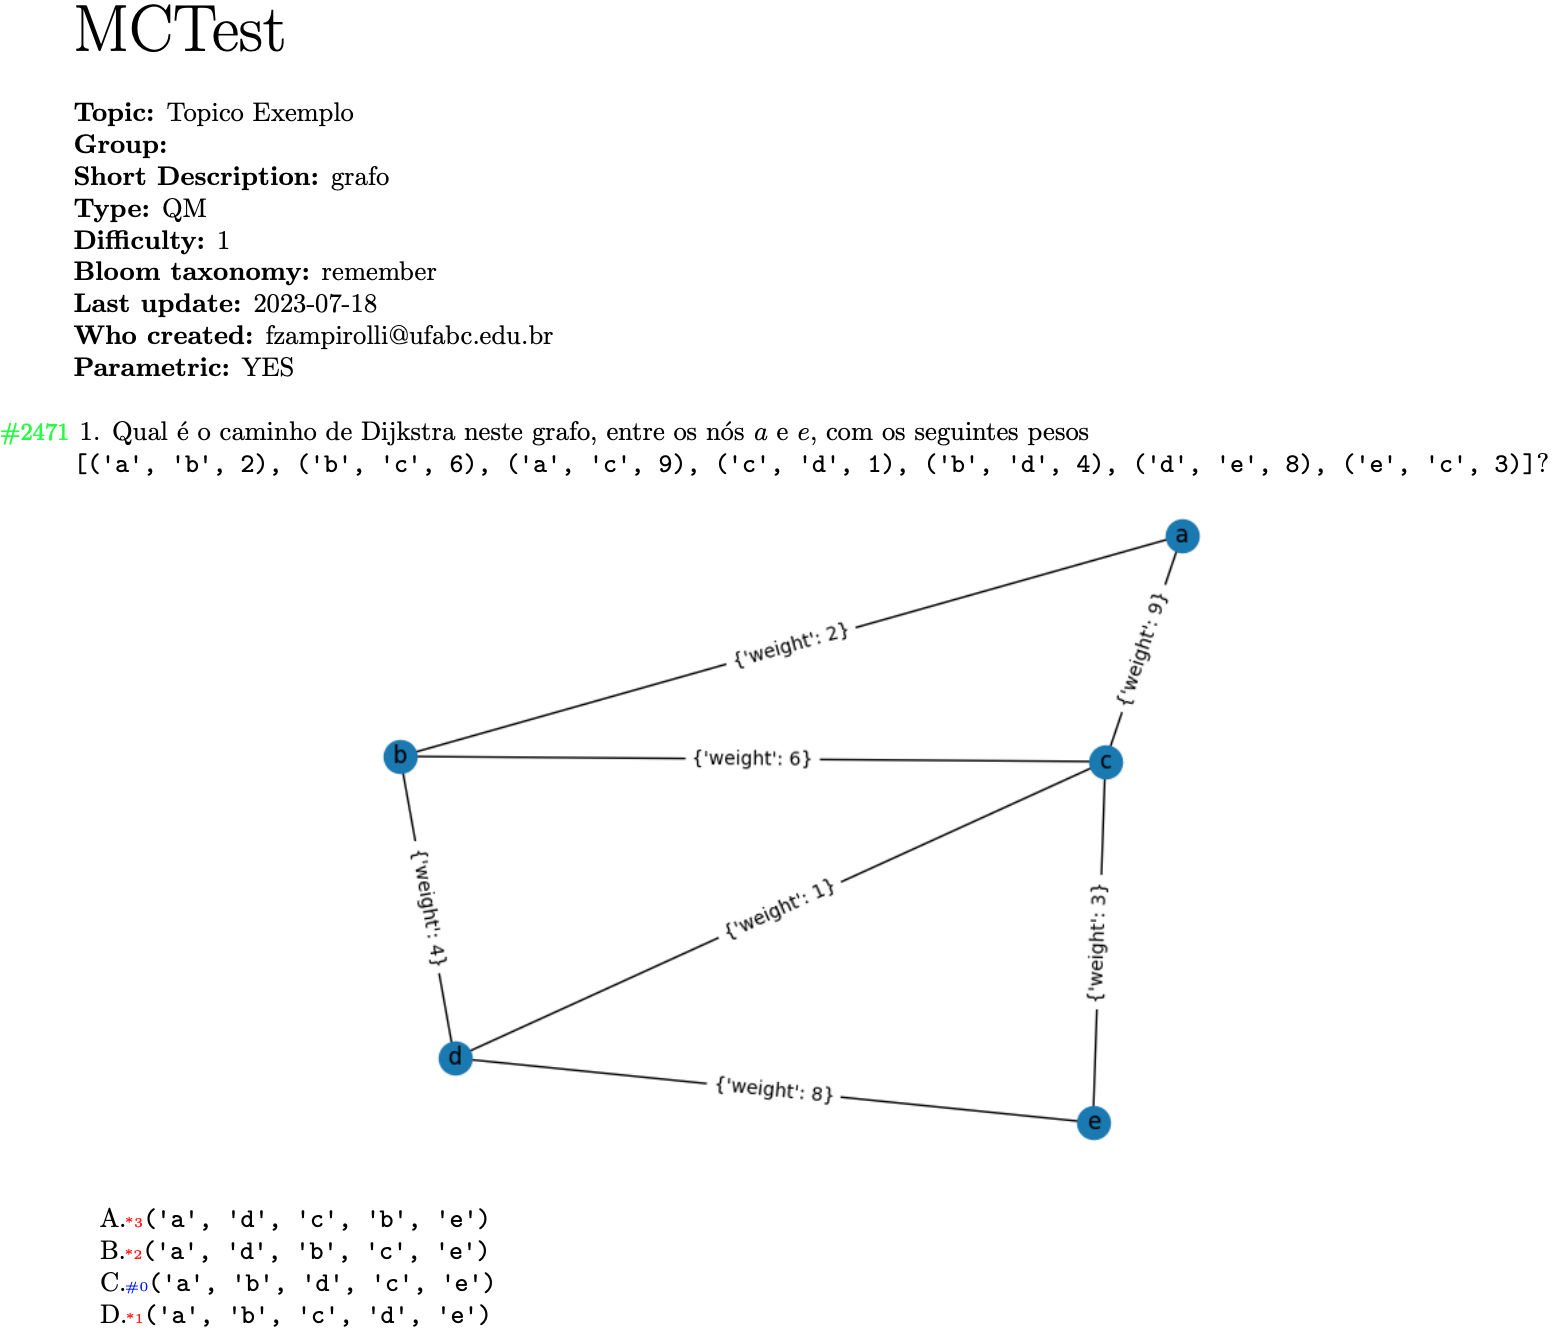
\includegraphics[width=0.9\textwidth]{cap12_questaoQM_grafoPDF.png}
  \caption{Recorte do PDF gerado para a questão paramétrica com grafo e figura referente ao Código \ref{lst:questaoQM_grafo}.}
  \label{fig:cap12_questaoQM_grafoPDF}
\end{figure}

\subsubsection{Questão paramétrica com matriz e figura}

No arquivo \verb|static/Utils.py|, localizado no GitHub \href{https://github.com/fzampirolli/mctest}{github.com/fzampirolli/mctest}, há vários métodos úteis para a criação de questões paramétricas. Um desses métodos é o \texttt{drawMatrix()}, que permite desenhar uma matriz, conforme serão demonstrados nos códigos desta seção.

\begin{listing}[!ht]
\begin{myboxCode}{corCodigo}{\textbf{Método: } desenha matriz}\vspace{3mm}
\hrule
\begin{minted}[xleftmargin=20pt,linenos=true]{python}
def drawMatrix(A, myfile):
    """
    Desenha uma representação visual de uma matriz e salva a imagem em um arquivo.
    Exemplo de uso:
    No enunciado da questão, desenhe a seguinte figura 
    (copie o código abaixo para uma nova questão):
    \begin{figure}[h!]
    \centering
    \includegraphics[scale=0.55]{[[code:f"./tmp/imgs180days/{pathGraficoA}"]]} 
    \end{figure}

    [[def:
    import numpy as np
    Lin, Col = 4, 5
    A = np.random.randint(10, size=(Lin, Col))
    # Plotagem da função
    import hashlib
    s =str([Lin, Col]) 
    h = hashlib.md5(s.encode()) # create hash - arquivo único
    h = str(h.hexdigest())
    fig0 = f'fz_figExample01{Lin}_{Col}_{h}.png'    
    drawMatrix(A, fig0)
    ]] """
    import matplotlib.pyplot as plt

    fig, ax = plt.subplots()
    mat = ax.imshow(A, cmap='Pastel1', interpolation='nearest')

    for x in range(A.shape[0]):
        for y in range(A.shape[1]):
            ax.annotate(str(A[x, y])[0], xy=(y, x), horizontalalignment='center', 
                        verticalalignment='center')

    plt.show()
    fig.savefig(f'./tmp/imgs180days/{myfile}.png', dpi=300)
    plt.close()
\end{minted}
\end{myboxCode}
\caption{Método para desenhar matriz.}
\label{lst:questaoDesenhaMatriz}
\end{listing}

% \tiny < \scriptsize < \footnotesize < \small < \normalsize < \large < \Large < \LARGE < \huge < \Huge

A questão apresentada nos Códigos \ref{lst:questaoMatrizRosaParte1} e \ref{lst:questaoMatrizRosaParte2} propõe a criação de um programa que manipula matrizes para identificar e ativar elementos com determinada condição em relação aos seus vizinhos. O programa recebe uma matriz de entrada \(E\) e cria uma matriz de saída \(F\), inicializada com o valor ``-1''. 
%
Um elemento \((i, j)\) da matriz \(E\) é considerado ``maior'' ou ``menor'' em relação aos seus vizinhos nas direções especificadas. As direções são codificadas numericamente conforme a tabela fornecida na questão (ver Figura \ref{fig:cap12_questaoMatrizRosaPDF}).
%
O programa deve percorrer a matriz de entrada \(E\) e, para cada elemento que atenda à condição de ser ``maior'' ou ``menor'' em relação aos seus vizinhos, o valor correspondente na matriz de saída \(F\) deve ser atualizado.
%
Após a ativação de todos os elementos que atendem à condição, o programa deve imprimir a matriz \(F\). Além disso, são fornecidos exemplos de uma matriz de entrada e a saída correspondente, exibidos na forma de imagens.
%
O programa deve conseguir lidar com matrizes de qualquer dimensão e garantir que os elementos de borda da matriz \(F\) sejam mantidos como ``-1''.
%
O exemplo fornecido mostra uma matriz de entrada e a matriz de saída resultante após a ativação dos elementos que atendem à condição especificada. As imagens mostram a representação gráfica das matrizes.
%
Para simplificar a resolução desta questão, é crucial destacar que \(a_0 = (i, j)\) não se encontra em um pixel de borda. Em outras palavras, na matriz \(F\), todos os elementos correspondentes às bordas devem ser mantidos com o valor ``-1''. Um exemplo da saída dessa questão pode ser observado na Figura \ref{fig:cap12_questaoMatrizRosaPDF}.


\begin{listing}[!ht]
\begin{myboxCode}{corCodigo}{\textbf{Questão: } }\vspace{3mm}
\hrule
{\footnotesize
\begin{minted}[xleftmargin=20pt,linenos=true]{python}
Um elemento \(a_0=(i,j)\) é de uma matriz dito ser \textbf{[[code:direcao]]
[[code:maiormenor]]} se seu valor é  [[code:maiormenor]] do que o valor de 
seus vizinhos nas direções [[code:direcao_viz]], considerando a seguinte
codificação para as possíveis direções: 
\
\begin{table}[h!]
\centering\vspace{-2mm}
\begin{tabular}{lllll}
\cline{1-3}
\multicolumn{1}{|l|}{\(a_8=\) Noroeste} & \multicolumn{1}{l|}{\(a_1=\) Norte}  & 
\multicolumn{1}{l|}{\(a_2=\) Nordeste} &  &  \\ \cline{1-3}
\multicolumn{1}{|l|}{\(a_7=\) Oeste}      & \multicolumn{1}{l|}{\(a_0=(i,j)\)} &
\multicolumn{1}{l|}{\(a_3=\) Leste}      &  &  \\ \cline{1-3}
\multicolumn{1}{|l|}{\(a_6=\) Sudoeste} & \multicolumn{1}{l|}{\(a_5=\) Sul}    & 
\multicolumn{1}{l|}{\(a_4=\) Sudeste}  &  &  \\ \cline{1-3}
\end{tabular}
\end{table}

\vspace{-2mm}
\noindent Faça um programa para criar e ler uma matriz de entrada \(E\) de inteiros. 
Seu programa deve criar também uma matriz de saída \(F\) e inicializa-la com o valor 
``-1''. Diz-se que um elemento \((i,j)\) de \(F\) é \emph{ativado} quando é atribuída a 
\(F[i,j]\) o valor de \(E[i,j]\), isto é, quando \(F[i,j] \leftarrow E[i,j]\). O 
seu programa deve também imprimir a matriz \(F\) depois de ativar todos os seus 
elementos que são \textbf{[[code:direcao]]  [[code:maiormenor]]}. Veja a seguir 
um exemplo \([[code:Linhas]] \times [[code:Colunas]]\) com a entrada e a saída 
correspondente. \\

\noindent {\bf Obs.:} considere \(a_0=(i,j)\) não pertencer a um pixel de borda, isto 
é, na matriz \(F\) todos os elementos de borda ficam com valor ``-1''. O seu programa 
deve funcionar para matrizes de quaisquer dimensões. 
 
\begin{table}[h!]\vspace{-4mm}
\begin{tabular}{cc}
\includegraphics[scale=0.56]{[[code:f"./tmp/imgs180days/{pathGraficoA}"]]}  &  
\includegraphics[scale=0.56]{[[code:f"./tmp/imgs180days/{pathGraficoB}"]]}  
\end{tabular}
\end{table}

\end{table}
\end{minted}
}
\end{myboxCode}
\caption{Questão paramétrica com matriz -- Parte 1: Descrição de questão.}
\label{lst:questaoMatrizRosaParte1}
\end{listing}


\begin{listing}[!ht]
\begin{myboxCode}{corCodigo}{\textbf{Questão: } }\vspace{3mm}
\hrule
{\footnotesize
\begin{minted}[xleftmargin=20pt,linenos=true]{python}
[[def:
import json, random, numpy as np

def direcoes(offset, dir):
  """ Método que retorna as direções adjacentes à direção dada. """
  dir1, dir2 = (dir - 1) % 8 + 1, (dir + 1) % 8 + 1
  return (dir1, dir, dir2)
    
# Parâmetros utilizados no enunciado da questão 
#>>>> BEGIN 
dir = random.choice([1,2,3,4,5,6,7,8])  
direcaoAll = ["Norte","Nordeste","Oeste","Sudeste","Sul","Sudoeste","Leste","Noroeste"]
direcao = direcaoAll[dir-1]

maiormenor = random.choice(["maior", "menor"])
m, n = random.randrange(7, 9, 1), random.randrange(15, 21, 1)
Linhas, Colunas = m, n

#direcoes  0      1      2     3     4     5      6      7       8
offset = [[0,0],[-1,0],[-1,1],[0,1],[1,1],[1,0],[1,-1],[0,-1],[-1,-1]]
(dir1,dir0,dir2) = direcoes(offset,dir)
direcao_viz = "$a_"+str(dir1)+"$, $a_"+str(dir0)+"$, $a_"+str(dir2)+"$"
#<<<< END 

A = (np.random.random((m, n)) * 10).astype(int)
B = (np.zeros(A.shape) - 1).astype(int)
for i in range(1, m - 1):
  for j in range(1, n - 1):
    if maiormenor == "menor":
      if (A[i + offset[dir1][0], j + offset[dir1][1]] > A[i, j]
        and A[i + offset[dir0][0], j + offset[dir0][1]] > A[i, j]
        and A[i + offset[dir2][0], j + offset[dir2][1]] > A[i, j]):
        B[i, j] = A[i, j]
    else:
      if (A[i + offset[dir1][0], j + offset[dir1][1]] < A[i, j]
        and A[i + offset[dir0][0], j + offset[dir0][1]] < A[i, j]
        and A[i + offset[dir2][0], j + offset[dir2][1]] < A[i, j]):
        B[i, j] = A[i, j]

import hashlib
s =''.join([str(i) for i in A.flatten()]) # 2d to 1d to str
h = hashlib.md5(s.encode()) # create hash - arquivo único
pathGrafico = 'figRosa(' + direcao + ')(' + maiormenor + ')(' + str(h.hexdigest()) + ')' 
pathGraficoA, pathGraficoB = pathGrafico + 'a.png', pathGrafico + 'b.png'

drawMatrix(A, pathGraficoA)
drawMatrix(B, pathGraficoB)
]]
\end{minted}
}
\end{myboxCode}
\caption{Questão paramétrica com matriz -- Parte 2: Bloco de código em Python.}
\label{lst:questaoMatrizRosaParte2}
\end{listing}

\begin{figure}[!ht]
  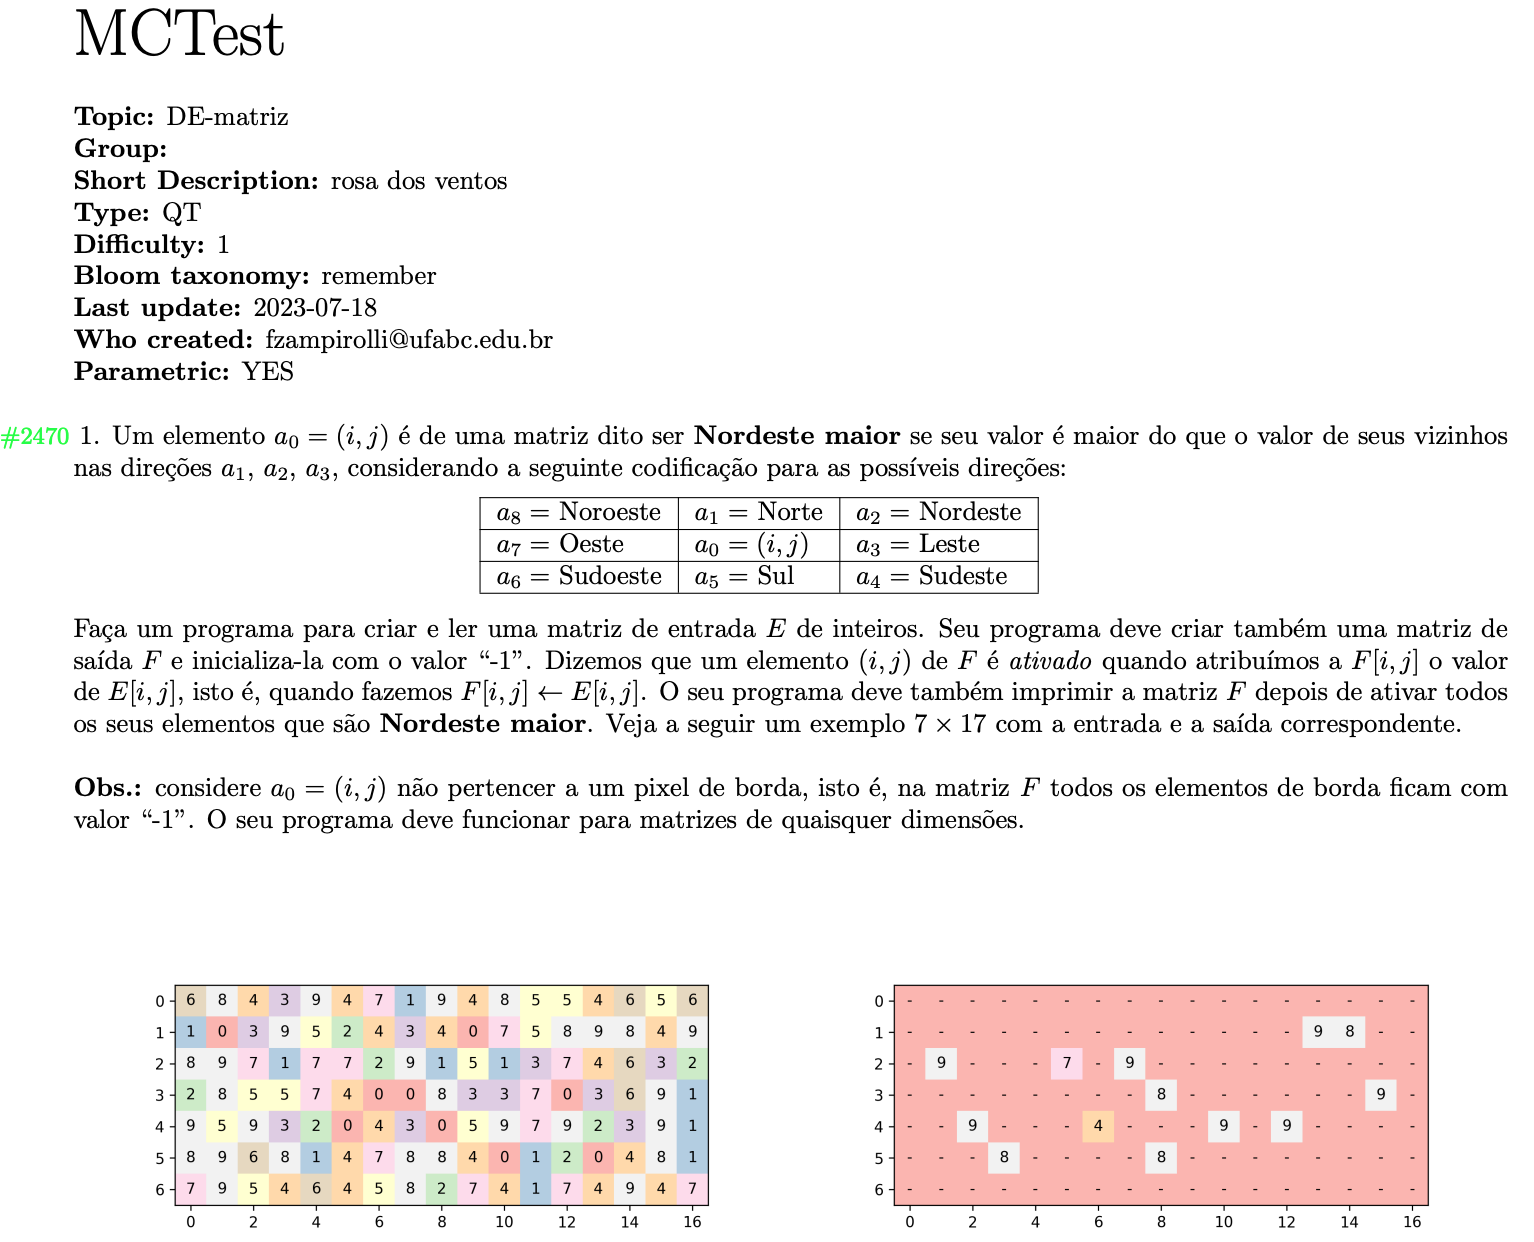
\includegraphics[width=0.9\textwidth]{cap12_questaoMatrizRosaPDF.png}
  \caption{Recorte do PDF gerado para a questão paramétrica com matriz criada pelos Códigos \ref{lst:questaoMatrizRosaParte1} e \ref{lst:questaoMatrizRosaParte2}.}
  \label{fig:cap12_questaoMatrizRosaPDF}
\end{figure}

\subsubsection{Resultados}

O MCTest foi aplicado na disciplina de Processamento da Informação. Os resultados indicam que o método é eficaz na geração de exames com variações nos textos, mantendo o mesmo conteúdo e nível de dificuldade. Além disso, os estudantes consideraram as questões claras e relevantes para o conteúdo da disciplina.

Foram apresentados três exemplos de questões paramétricas, mas a quantidade de tipos e variações está diretamente relacionada à criatividade do professor que as prepara.

%%%%%%%%%%%%%%%%%%%%%%%%%%%%%%%%%%%%%%%%%%%%%%%%%%%%%%%%%%%%%%%%%%%%%%%%%
\subsection{Artigo descrevendo o MCTest em conjunto com \textit{Google Forms} e \textit{Google Sheets}}\label{sec:experMCTestForms}
%%%%%%%%%%%%%%%%%%%%%%%%%%%%%%%%%%%%%%%%%%%%%%%%%%%%%%%%%%%%%%%%%%%%%%%%%


O artigo de \citeonline{2020:Zampirolli.Batista.ea} aborda a adaptação do MCTest para solucionar o problema de avaliação a distância durante a pandemia. A solução permite criar questões paramétricas com Python e \LaTeX. A correção automática é feita com o \textit{Google Forms} e \textit{Google Sheets}, constituindo uma contribuição original. A solução adaptada foi aplicada com sucesso em uma turma de Cálculo 1 com 100 estudantes.

\subsubsection{Método}

O MCTest permite a geração eficiente de QTs ou de QMs que podem ser modificadas parametricamente, produzindo muitas variações dessas questões. Isso é realizado por meio de várias bibliotecas da linguagem de programação Python, com as quais o MCTest calcula respostas automaticamente. O MCTest tem a vantagem de permitir questões paramétricas criadas com \LaTeX{} e Python, com exemplos de uso apresentados no artigo e reproduzidos nesta seção.

O artigo descreve um desafio enfrentado na adaptação do MCTest para avaliações \textit{online} durante a pandemia, já que o sistema originalmente gerava exames em papel para serem aplicados em sala de aula. Para solucionar esse desafio, os autores propõem uma solução adaptada do MCTest que gera exames e os envia por e-mail aos estudantes em formato PDF, com submissões realizadas em uma planilha do \textit{Google Forms} preenchida pelos estudantes e compilada ao professor em uma planilha do \textit{Google Sheets}.

A planilha do \textit{Google Sheets} é adaptada para a correção automática, conforme apresentado na Figura \ref{fig:cap12_examesSheets_planilha}. Esta planilha também está disponível em \href{https://github.com/fzampirolli/mctest}{github.com/fzampirolli/mctest}, no arquivo \verb|static/MCTest_Forms.ods|. A nota do estudante é calculada com base nas respostas enviadas, na chave de respostas armazenada na aba \verb|templateAV1| e nas variações sorteadas para cada estudante na aba \verb|variationsAV1|. A identificação, nome e e-mail de cada estudante são armazenados na aba \verb|listStudents|. Todas essas abas são preenchidas com cópias dos arquivos enviados pelo MCTest, exemplificados a seguir. A pontuação é calculada para cada questão, incluindo uma QT com resposta exata, nas colunas H e I (Q4 e Q5, respectivamente). Os autores explicam em detalhes como a correção automática é realizada nas planilhas do \textit{Google Sheets}, incluindo a correção manual pelo professor para avaliar a demonstração da resposta exata apresentada pelo estudante para essa QT.

Os autores estenderam o código do MCTest para permitir a correção automática de QTs, incluindo a possibilidade do professor receber dois arquivos CSV: um com as chaves de respostas para cada questão e outro com o número da variação enviada para cada estudante. Além disso, o código foi adaptado para permitir a criação de QTs com respostas paramétricas exatas, inseridas em um arquivo CSV e posteriormente na planilha do \textit{Google Sheets}. Os autores apresentam exemplos de QMs e QTs, como a apresentada na Seção \ref{sec:equacao_sympy_figura} -- \nameref{sec:equacao_sympy_figura}, e explicam em detalhes como o MCTest lida com questões paramétricas e a correção automática de QTs. Um exemplo de QT exata foi apresentado no Código \ref{lst:questaoQT_exata}.

\begin{figure}[!ht]
\centering
  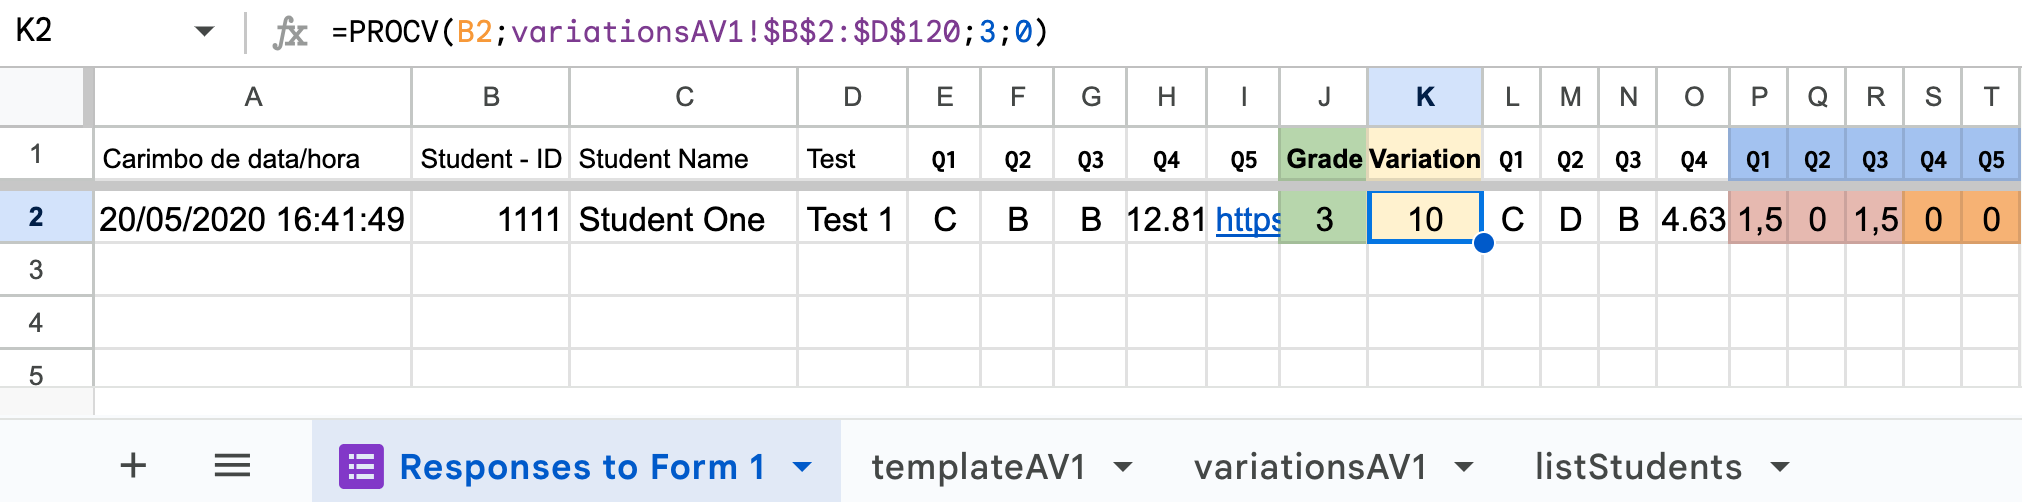
\includegraphics[width=0.9\textwidth]{cap12_examesSheets_planilha.png}
  \caption{Planilha mostrando o questionário preenchido de um estudante. Adaptado de \citeonline{2020:Zampirolli.Batista.ea}.}
  \label{fig:cap12_examesSheets_planilha}
\end{figure}

\begin{myboxCode}{corCSV}{\textbf{Arquivo CSV copiado na aba \texttt{templateAV1}, com os gabaritos. Ver explicações na Seção \ref{sec:QMgabarito} -- \nameref{sec:QMgabarito} (as colunas são separadas por vírgula)}}\vspace{3mm}
\hrule
{\footnotesize
\begin{verbatim}
variation Q1 Q2 Q3 Q4    Q5
1         C  E  D  3.47   
2         B  D  B  3.99  
3         A  B  C  4.07  
4         D  E  C  4.11  
5         E  B  A  4.29  
6         E  A  C  3.94  
7         B  B  D  3.56  
8         B  B  D  4.16  
9         B  E  B  3.73  
10        C  D  B  4.63  
\end{verbatim}
}
\end{myboxCode}


\begin{myboxCode}{corCSV}{\textbf{Arquivo CSV copiado na aba \texttt{variationsAV1}, com os estudantes. Ver explicações na Seção \ref{sec:exameQM_QT_criarPDF} -- \nameref{sec:exameQM_QT_criarPDF}}}\vspace{3mm}
\hrule
{\footnotesize
\begin{verbatim}
Room    ID  Name         Variation
Room1 1111  Student One         10
Room1 2222  Student Two          8
\end{verbatim}
}
\end{myboxCode}

\begin{myboxCode}{corCSV}{\textbf{Arquivo CSV copiado na aba \texttt{listStudents}, com as variações. Ver explicações na Seção \ref{sec:professorCriarTurma} -- \nameref{sec:professorCriarTurma}}}\vspace{3mm}
\hrule
{\footnotesize
\begin{verbatim}
1111  Student One  student1@email.com
2222  Student Two  student2@email.com
\end{verbatim}
}
\end{myboxCode}


\subsubsection{Experimentos}

Os autores aplicaram o MCTest em uma turma da disciplina de Cálculo 1 na Universidade Federal do ABC, composta por 100 estudantes. A disciplina é parte do Bacharelado em Ciência e Tecnologia e possui alta taxa de reprovação. Durante sete semanas, os estudantes assistiram às aulas \textit{online} e fizeram dois testes formativos, cada um contendo cinco questões paramétricas, duas QTs e três QMs. Os testes foram dados no mesmo formato do modelo apresentado na Figura \ref{fig:cap12_examesPDF_MCTestS}, com questões e alternativas sorteadas. O Teste 1 foi aplicado \textit{online} e os estudantes tiveram 24 horas para responder. O Teste 2, assim como o Exame 1, foram mais complexos e contaram para a nota final. Os estudantes tiveram dificuldades nas QTs, mas obtiveram bom desempenho nas QMs. A taxa de erros foi baixa nos testes e exames, e os estudantes não relataram problemas técnicos na submissão das respostas. Os autores suspeitam que a facilidade de acesso a recursos \textit{online} possa ter influenciado no desempenho dos estudantes nas QTs. Para manter os estudantes engajados, o professor aplicou um terceiro exame contendo apenas QTs com submissão de imagens digitalizadas das respostas manuscritas.

\begin{figure}[!ht]
\centering
  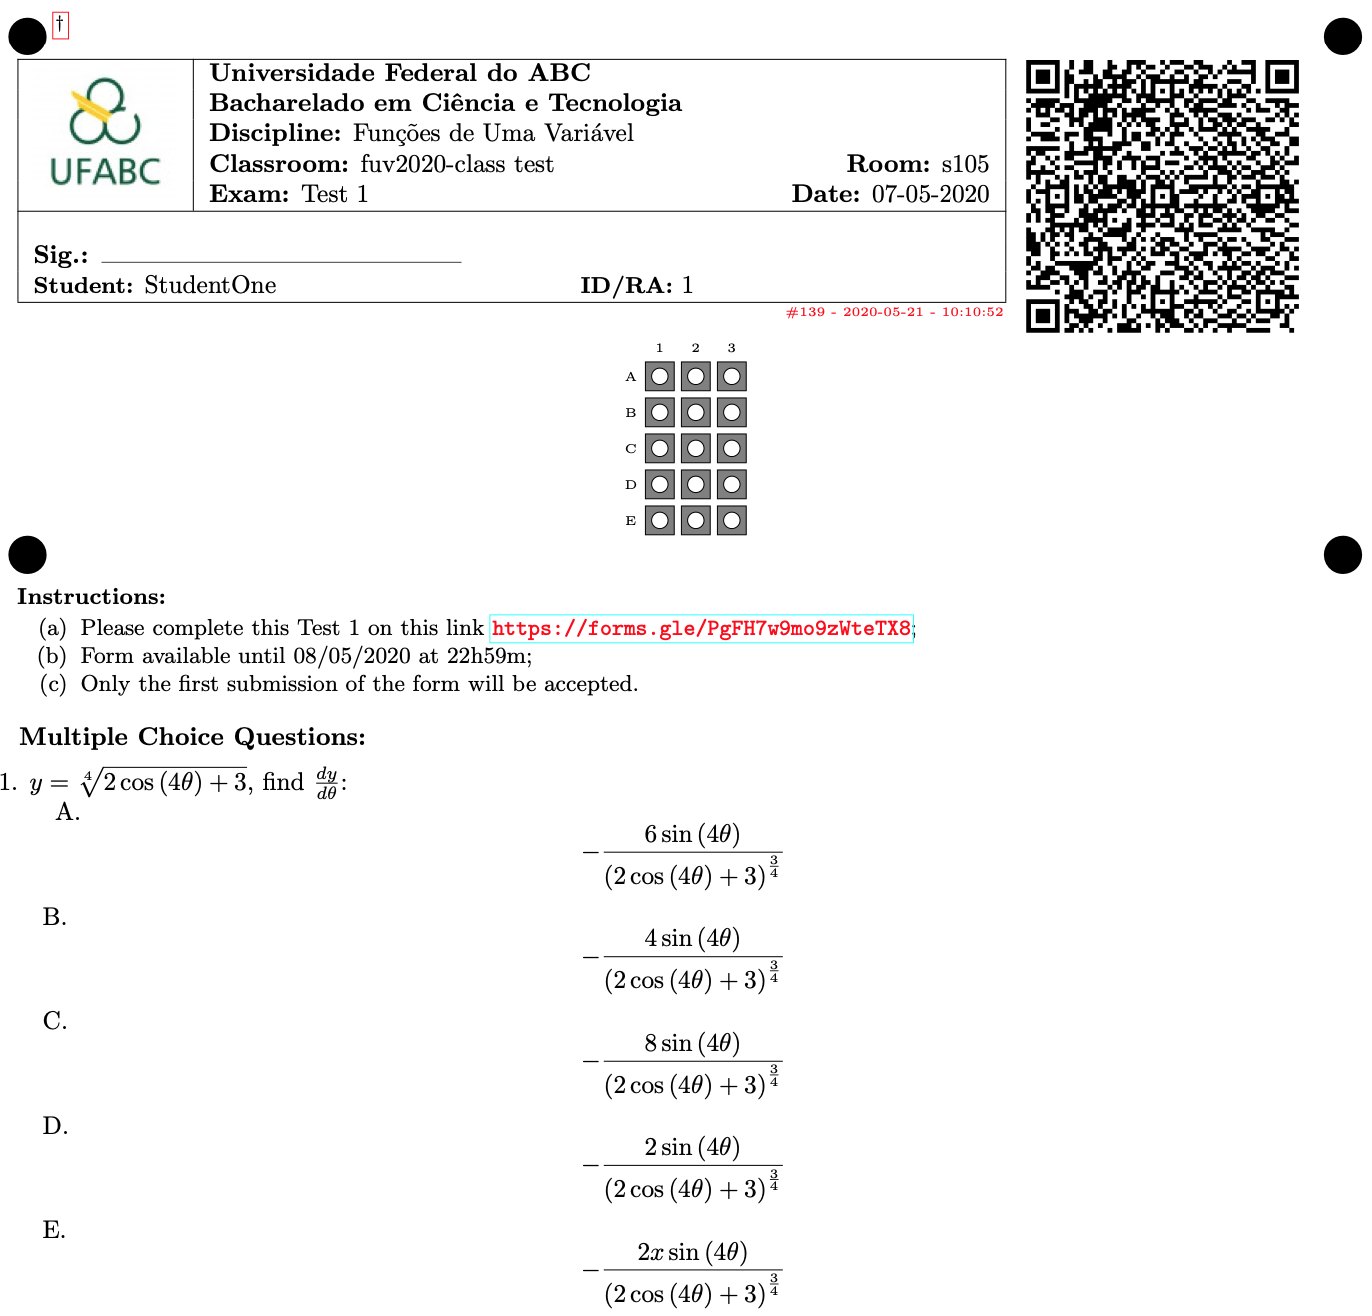
\includegraphics[width=0.9\textwidth]{cap12_examesPDF_MCTestS.png}
  \caption{Exemplo de exame utilizado em Cálculo 1. Adaptado de \citeonline{2020:Zampirolli.Batista.ea}.}
  \label{fig:cap12_examesPDF_MCTestS}
\end{figure}

Os autores abordam a questão do plágio em contextos \textit{online} e propõem medidas preventivas, incluindo a administração de exames individualizados, a imposição de restrições temporais e a supervisão por meio de \textit{webcams}. Contudo, eles reconhecem que em circunstâncias extraordinárias, como a pandemia, torna-se necessário empregar ferramentas que viabilizem as atividades de aprendizado, como mencionado no artigo.

Os resultados dos experimentos mostraram ser importante elaborar questões \textit{online} com enunciados melhor elaborados para os estudantes poderem raciocinar para achar as soluções e não achar respostas prontas na internet.
%
Os autores destacam que o MCTest pode ser uma ferramenta valiosa para manter os estudantes engajados em atividades com QMs e sugerem a aplicação de vários exames desse tipo, com correção automática, para estimular a participação dos estudantes.

%%%%%%%%%%%%%%%%%%%%%%%%%%%%%%%%%%%%%%%%%%%%%%%%%%%%%%%%%%%%%%%%%%%%%%%%%
\subsection{Artigo descrevendo a adoção de QMs com \ pesos diferentes \ nas \ alterna\-tivas}
%%%%%%%%%%%%%%%%%%%%%%%%%%%%%%%%%%%%%%%%%%%%%%%%%%%%%%%%%%%%%%%%%%%%%%%%%

O artigo de \citeonline{2021:Zampirolli.Batista.ea*2} apresenta uma adaptação do sistema MCTest que permite a avaliação automatizada de QMs com respostas ponderadas. 

\subsubsection{Método}

O sistema MCTest original produz um arquivo CSV que inclui as respostas para cada QM, com as pontuações atribuídas a cada alternativa. A adaptação proposta neste artigo introduz uma coluna adicional no arquivo de respostas para cada questão, indicando o peso de cada alternativa. O sistema de avaliação automática calcula a nota do estudante ponderando a pontuação de cada alternativa de acordo com seu respectivo peso.

O processo de criação de questões e exames é o mesmo apresentado nos capítulos anteriores. A diferença está na forma de calcular a nota do estudante. Esta seção detalhará esse processo.

A planilha utilizada no artigo disponível no GitHub, em \href{https://github.com/fzampirolli/mctest}{github.com/fzampirolli/mctest}, no arquivo \verb|static/GRADE.ods|.
%
Essa planilha possui duas abas principais. A primeira é a aba BD, contendo as correções geradas pelo MCTest ao submeter os exames digitalizados, conforme visualizado na Figura \ref{fig:cap12_examesMCTest_pesos_BD}. A segunda aba é para o cálculo da nota final, como apresentado na Figura \ref{fig:cap12_examesMCTest_pesos_Final}.

\begin{figure}[!ht]
\centering
  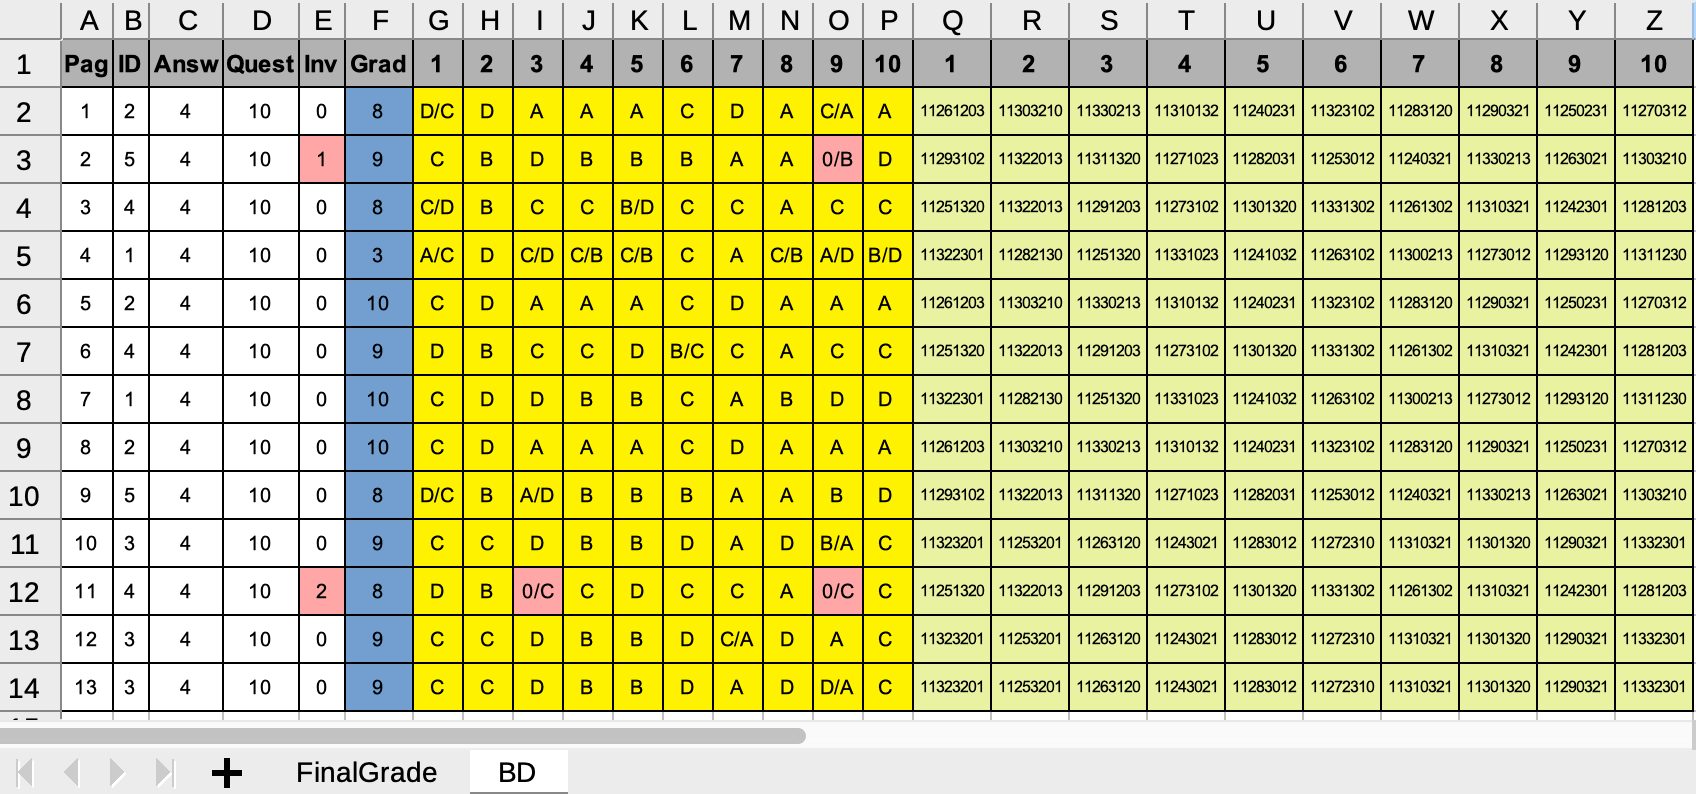
\includegraphics[width=1\textwidth]{cap12_examesMCTest_pesos_BD.png}
  \caption{Visualização do arquivo CSV com as correções. Adaptado de \citeonline{2021:Zampirolli.Batista.ea*2}.}
  \label{fig:cap12_examesMCTest_pesos_BD}
\end{figure}

\begin{figure}[!ht]
\centering
  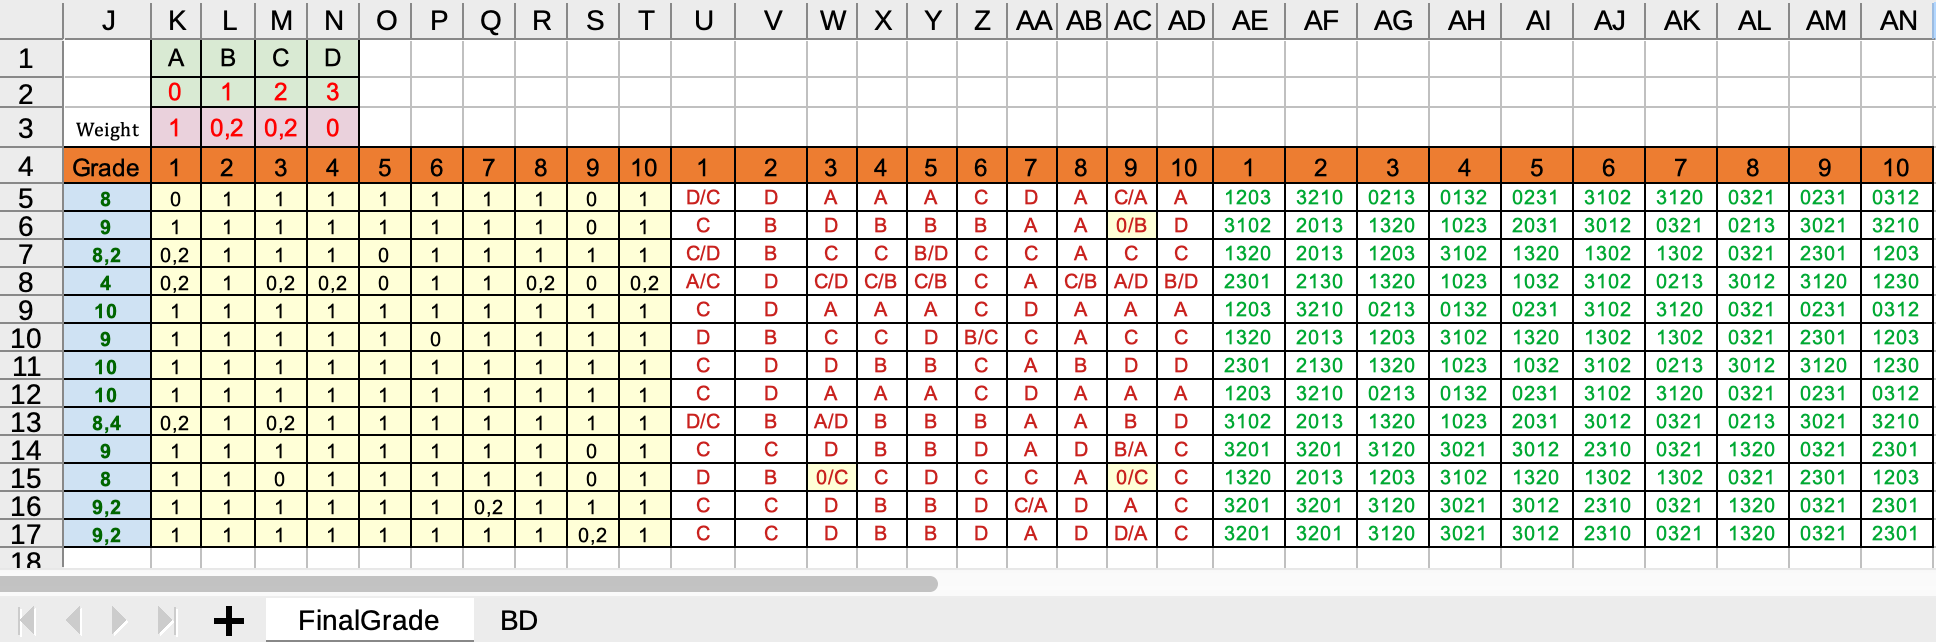
\includegraphics[width=1\textwidth]{cap12_examesMCTest_pesos_Final.png}
  \caption{Cálculo final do exame. Adaptado de \citeonline{2021:Zampirolli.Batista.ea*2}.}
  \label{fig:cap12_examesMCTest_pesos_Final}
\end{figure}

Na Figura \ref{fig:cap12_examesMCTest_pesos_BD}, as colunas Q a Z na planilha mostram o ID da questão no BD e a ordem das alternativas sorteadas para os estudantes. A célula Q2, por exemplo, possui o valor 11261203, em que  1126 é o ID da questão e 1203 indica a ordem das alternativas sorteadas (A=1, B=2, C=0, D=3). Com fórmulas simples, é possível calcular a nota final atribuindo pesos às alternativas. Na Figura \ref{fig:cap12_examesMCTest_pesos_Final}, o peso da alternativa correta é 1, as parcialmente corretas têm peso 0,2 cada e a alternativa absurda tem peso 0. O campo amarelo na Figura \ref{fig:cap12_examesMCTest_pesos_Final} exibe a pontuação de cada questão, em que cada linha corresponde ao QR de um estudante. A nota total do estudante para o exame é calculada somando as notas de cada questão.

O sistema MCTest pode ser usado para avaliar exames realizados em formato físico ou \textit{online}. No caso de exames realizados em formato físico, os estudantes respondem às questões em um QR impresso, como apresentado na Figura \ref{fig:cap12_examesPDF_MCTestS}. O QR impresso é então digitalizado e o sistema MCTest é usado para corrigir as respostas. No caso de exames realizados em formato \textit{online}, os estudantes respondem às questões em um navegador da web, como descrito na Seção \ref{sec:experMCTestForms} -- \nameref{sec:experMCTestForms}. 

\subsubsection{Experimentos}

O método deste artigo foi aplicado a exames realizados em formato físico ou \textit{online} e validado com um total de 607 estudantes de três diferentes disciplinas: Redes e Comunicações, Natureza da Informação e Compiladores. Os resultados mostraram que o sistema de correção automática é preciso e confiável. O sistema foi bem avaliado pelos estudantes, que o consideraram uma ferramenta útil para a avaliação de seus conhecimentos.

%%%%%%%%%%%%%%%%%%%%%%%%%%%%%%%%%%%%%%%%%%%%%%%%%%%%%%%%%%%%%%%%%%%%%%%%%
\subsection*{Artigo comparando diferentes processos seletivos na EPUFABC}
%%%%%%%%%%%%%%%%%%%%%%%%%%%%%%%%%%%%%%%%%%%%%%%%%%%%%%%%%%%%%%%%%%%%%%%%%

O artigo de \citeonline{2021:Zampirolli.Batista.ea} analisa o processo de seleção para a Escola Preparatória da UFABC (EPUFABC) aplicado a milhares de candidatos de escolas públicas da região. A EPUFABC oferece um curso gratuito voltado exclusivamente para estudantes de baixa renda que se inscreverão em exames de entrada na universidade. O processo de seleção emprega a Teoria Clássica ao Item (TCI), mas há dúvidas sobre a imparcialidade dos critérios de desempate. Por isso, os autores contrastam a abordagem atual do processo com a Teoria da Resposta ao Item (TRI) \cite{birnbaum1968some}. Os resultados mostram que o método TRI pode melhorar substancialmente o processo de seleção do EPUFABC.

O artigo menciona que o exame de entrada da Universidade de São Paulo (USP) é um exemplo de seleção desafiadora, com inúmeros candidatos para poucas vagas. Para exames com alta taxa de inscrição, lidar com a nota de corte, na qual muitos candidatos provavelmente terão pontuação igual, é um desafio.

Para resolver esse problema, o Exame Nacional do Ensino Médio (ENEM) no Brasil passou a utilizar a Teoria da Resposta ao Item (TRI) desde 2009. A TRI também é empregada em outros países, como nos Estados Unidos, em exames como o TOEFL.

\subsubsection*{Método}

Os autores foram inspirados pela metodologia do ENEM e avaliaram o processo de seleção utilizado pela EPUFABC, que atende a milhares de candidatos desde 2010. O exame de admissão da EPUFABC é composto por 10 QMs para cada área de conhecimento, além de um exame de Gramática Portuguesa, que substitui a redação exigida pelo ENEM. As áreas avaliadas são: Ciências Humanas, Ciências da Natureza, Línguas e Códigos (Inglês-Espanhol-Português) e Matemática.

A avaliação comparou o Processo de Seleção do EPUFABC aplicado de 2019 a 2021 com o ENEM, que adota o modelo logístico de três parâmetros da TRI. Foram desenvolvidos três \textit{scripts} em Python e R no \textit{Google Colab} para realizar as análises. Cada \textit{script} passa por três etapas: pré-processamento, geração da matriz de respostas (em Python) e análise estatística (em R). Todos os dados utilizados no artigo podem ser baixados em \href{http://vision.ufabc.edu.br/MCTest/public/IRT2021}{vision.ufabc.edu.br/MCTest/public/IRT2021}, que inclui todos os arquivos CSV utilizados pelos Notebooks, mas sem a identificação dos candidatos.

Para comparações, foram utilizados também os microdados do ENEM de 2019 disponibilizados pelo Ministério da Educação. Os dados do ENEM requerem um pré-processamento complexo devido ao seu tamanho, envolvendo segmentação, extração de colunas relevantes e geração de matrizes de respostas.

\subsubsection{Experimentos}

Este estudo baseia-se em três conjuntos de dados: (1) MCTest (2019 e 2020), (2) Moodle (2021) e (3) ENEM (2019). Tanto a Teoria Clássica ao Item (TCI) quanto a Teoria da Resposta ao Item (TRI) foram utilizadas para analisar e comparar os resultados.

Os exames TCI de 2019 e 2020 foram realizados presencialmente em um sábado, com 50 QMs nas cinco áreas de conhecimento referidas anteriormente. Os exames foram corrigidos automaticamente pelo sistema MCTest, conforme explicado no Capítulo \ref{ch:examesQR} -- \nameref{ch:examesQR}. Em 2021, devido à pandemia de COVID-19, o processo de seleção foi adaptado para exames \textit{online}, realizados ao longo de cinco dias. Os candidatos acessaram material de ensino (videoaulas) e QMs na plataforma Moodle e tiveram 24 horas para responder. A pontuação final considerou o número de respostas corretas, presença nos cinco dias de exame e idade do candidato.

Em 2019, houve 2.033 candidatos no TCI, enquanto em 2020 houve 2.043 candidatos. Em ambos os anos, 633 candidatos foram selecionados para a EPUFABC, sendo metade para aulas no período da tarde e a outra metade no período da noite. 

No exame de 2021, os candidatos realizaram o exame \textit{online} na plataforma Moodle, totalizando 2.768 participantes. A EPUFABC ofereceu 380 vagas para o ano de 2021, sendo 190 vagas para cada período, e as aulas foram disponibilizadas remotamente na plataforma Moodle.

Foram calculadas médias e desvios padrão para os exames de todas as áreas de conhecimento dos processos TCI2019, TCI2020 e ENEM2019. As análises também incluíram Curvas Características do Item (CCI) da TRI. A comparação entre TCI e TRI mostrou que o método TRI pode ser útil como critério de desempate em processos de seleção, já que considera a habilidade do candidato em responder corretamente às questões.

O estudo também destacou a melhora significativa nas notas dos candidatos no TCI2021, que foi realizado \textit{online} com mais tempo disponível para responder às questões, em comparação com os processos presenciais anteriores. As análises mostraram que as habilidades dos candidatos em TCI2021, representadas pelas curvas CCI, estavam mais concentradas no lado direito da escala, indicando que candidatos com habilidades menores conseguiram acertar mais questões devido ao tempo extra para responder cada exame.


Após a continuidade deste trabalho, outro artigo de \citeonline{2021:Zampirolli.Junior.ea} foi publicado, descrevendo o desenvolvimento de um sistema interativo chamado ENEM interativo e disponível em \href{http://mctest.ufabc.edu.br:8000/ENEM}{mctest.ufabc.edu.br:8000/ENEM}. Esse sistema permite que os estudantes utilizem exames antigos do ENEM e os microdados disponibilizados pelo INEP para estudo.
%
No ENEM Interativo, os exames em formato PDF são convertidos para HTML e, automaticamente, botões de resposta são incorporados para cada questão. Ao finalizar cada exame, o botão de estatísticas abre uma nova página que apresenta informações como o gabarito, as respostas dos estudantes, as habilidades (valores fornecidos pelo INEP) e gráficos.
%
O sistema proporciona uma plataforma mais interativa e acessível para os estudantes explorarem exames anteriores do ENEM e analisarem seu desempenho em detalhes, incluindo informações estatísticas relevantes para a compreensão de seu progresso e habilidades.


\section{Considerações finais}

Neste capítulo, foram discutidas as versões 4 e 5 do MCTest, assim como os artigos que as acompanharam. Ao longo do tempo, o MCTest passou por uma significativa evolução, saindo de suas primeiras versões focadas em exames impressos e se tornando uma versão web atual, integrada também ao Moodle. Essa transformação trouxe diversos benefícios e avanços para o sistema.

Os experimentos e casos de uso apresentados nos artigos destacaram a aplicabilidade bem-sucedida do MCTest em diversas situações reais de ensino. Isso reforça a eficiência e versatilidade do sistema em diferentes contextos, abrangendo exames presenciais, \textit{online}, individualizados e integração com plataformas como o \textit{Google Forms}. Esse recurso mostrou-se especialmente relevante durante a pandemia de COVID-19, permitindo a continuidade da avaliação educacional mesmo em cenários remotos.

O MCTest-4 é um software desenvolvido para a correção de exames com QMs. Ele automatiza o processo de correção, gerando resultados precisos e poupando tempo dos educadores. Já o MCTest-4.G foi criado para a geração de exames com QMs, permitindo a criação de exames distintos e aleatórios para cada estudante, proporcionando maior segurança na aplicação dos exames.

A versão mais recente, o MCTest-5, é considerada um software web altamente funcional. Além de possuir as funcionalidades do MCTest-4, o MCTest-5 permite a criação, correção e compartilhamento de questões, apresentando recursos avançados e integração com outras plataformas educacionais, como o Moodle. No próximo capítulo, serão destacadas especialmente as especificidades das questões que envolvem EPs integrados ao \textit{plugin} VPL do Moodle.

Por fim, é relevante ressaltar que a maioria das publicações efetuadas nesta versão web do MCTest foram subsidiadas pelo projeto FAPESP, sob o processo \href{https://bv.fapesp.br/pt/auxilios/105047/um-sistema-universal-para-geracao-e-correcao-automatica-de-questoes-parametrizadas}{2018/23561-1}, cujo título é ``Um sistema universal para a geração e correção automática de questões parametrizadas''.

